%%%%%%%%%%%%%%%%%%%%%%%%%%%%%%%%%%%%%%%%%%%%%%%%%%%%%%%%%%%%%%%%%%%%%
% In English:
%    This is a Latex template for São Paulo Research Foudation (FAPESP)
%         reports (annual or final).
%    This is the modified version of the original Latex template from
%         following website.
%    Original Source: http://www.howtotex.com
%    For information about FAPESP, check http://www.fapesp.br/en
%    This template targets mainly on reports in Portuguese language.
%    New additions and changes in the latest version:
%        - Added the possibility of including multiple members in the
%          research team, with the commands \memberA{Name of Member A}
%          \memberB{Name of Member B} \memberC{Name of Member C} etc.
%        - Included commands to define project modality and the research
%          agency (if you want to use the same model for other research
%          agencies such as CAPES, CNPq etc).
%
% In Portuguese:
%    Este é um modelo Latex para relatórios (anual ou final) da Fundação
%         de Amparo à pesquisa do Estado de São Paulo (FAPESP).
%    Esta é uma versão modificada do modelo Latex do site supra mencionado.
%    Para informações sobre a FAPESP, verifique http://www.fapesp.br
%    Esse modelo foca principalmente nos relatórios escritos em Português.
%    Novas adições e alterações na última versão:
%       - Foi adicionada a possibilidade de incluir vários membros no
%         grupo de pesquisas, com os comandos \membroA{Nome do Membro A}
%         \membroB{} \membroC{} etc.
%       - Foram incluídos comandos para definir modalidade de projeto e
%         agência de fomento (caso queira utilizar o mesmo modelo para
%         outras agências, CAPES, CNPq etc).
%
% Author/Autor: André Leon Sampaio Gradvohl, Dr.
% Email:        andre.gradvohl@gmail.com
% Lattes CV:    http://lattes.cnpq.br/9343261628675642
% GitHub: http://gradvohl.github.io/
%
% Last update/Última versão: 19/Feb/2018
%
%%%%%%%%%%%%%%%%%%%%%%%%%%%%%%%%%%%%%%%%%%%%%%%%%%%%%%%%%%%%%%%%%%%%%%
\documentclass[12pt]{report}
\usepackage[a4paper]{geometry}
\usepackage[utf8]{inputenc}
\usepackage[english]{babel}
\usepackage[myheadings]{fullpage}
\usepackage[T1]{fontenc}
\usepackage{fancyhdr}
\usepackage{setspace}
\usepackage{sectsty}
\usepackage{url}

%%% iniciar capitulo na mesma pagina (Mateus) %%%
\usepackage{etoolbox}
\makeatletter %inicio da modificacao (iniciar capitulo na msma pag)
\patchcmd{\chapter}{\if@openright\cleardoublepage\else\clearpage\fi}{}{}{}
\makeatother %fim da modificacao
%%% iniciar capitulo na mesma pagina (Mateus) %%%

%%------
%% Comandos gerais
%% Observação: o arquivo "comandos.tex" tem que estar presente.
%%------
%%%%%%%%%%%%%%%%%%%%%%%%%%%%%%%%%%%%%%%%%%%%%%%%%%%%%%%%%%%%%%%%%%%%%
% In English:
%    This is a list of commands specification for FAPESP reports.
%
% In Portuguese:
%    Esta é uma lista de especificação de comandos para relatórios
% da Fundação de Amparo à pesquisa do Estado de São Paulo (FAPESP).
%
% Author/Autor: André Leon Sampaio Gradvohl, Dr.
% Email:        andre.gradvohl@gmail.com
% Lattes CV:    http://lattes.cnpq.br/9343261628675642
%
% Last update/Última versão: 11/Sep/2016
%%%%%%%%%%%%%%%%%%%%%%%%%%%%%%%%%%%%%%%%%%%%%%%%%%%%%%%%%%%%%%%%%%%%%%

\newcommand{\HRule}[1]{\rule{\linewidth}{#1}}
\setcounter{tocdepth}{3}
\setcounter{secnumdepth}{3}

\newcommand{\titulo}[1]{\def\meuTitulo{#1}}
\newcommand{\tituloIngles}[1]{\def\meuTituloIngles{#1}}
\newcommand{\numProjeto}[1]{\def\numFAP{#1}}
\newcommand{\tipoRelatorio}[1]{\def\tipoRelat{#1 }} %o espaço depois do #1 é importante
\newcommand{\modalidadeProjeto}[1]{\def\modProjeto{#1}}
\newcommand{\agFomento}[2]{\def\agFom{#1} \def\siglaAgFom{#2}} %extenso Sigla
\newcommand{\autor}[1]{\def\nomeAutor{#1}}
\newcommand{\cidade}[1]{\def\nomeCidade{#1}}
\newcommand{\universidade}[1]{\def\nomeUniversidade{#1}}
\newcommand{\faculdade}[1]{\def\nomeFaculdade{#1}}
\newcommand{\periodoVigencia}[1]{\def\periodVig{#1}}
\newcommand{\periodoRelatorio}[1]{\def\periodRelat{#1}}
\newcommand{\orientador}[1]{\def\nomeOrientador{#1}}

\newcommand\namegroup[3]{%
   \begin{minipage}[t]{0.4\textwidth}
   \hspace{0.6cm}
   \begin{tikzpicture}
   \node[anchor=south east,inner sep = 0](signF){\includegraphics[width=#3]{#2}};
   \end{tikzpicture}
   \vspace*{0.1cm}  % leave some space above the horizontal line
   \hrule
   \vspace{1mm} % just a bit more whitespace below the line
   \centering
   \begin{tabular}[t]{c}
   #1
   \end{tabular}
   \end{minipage}}

\author{}
\date{}

%Definição de membros da equipe de pesquisas
\newcommand{\membroA}[1]{\def\nomeMembroA{#1}}
\newcommand{\membroB}[1]{\def\nomeMembroB{#1}}
\newcommand{\membroC}[1]{\def\nomeMembroC{#1}}
\newcommand{\membroD}[1]{\def\nomeMembroD{#1}}
\newcommand{\membroE}[1]{\def\nomeMembroE{#1}}
\newcommand{\membroF}[1]{\def\nomeMembroF{#1}}

\newcommand{\Figure}[1]{Figura~\ref{fig:#1}}
\newcommand{\Table}[1] {Tabela~\ref{#1}}
\newcommand{\Equation}[1] {Equa\c{c}\~ao~\ref{#1}}
\newcommand{\addFigure}[3] { %Parametros scale, fig_name, caption
    \begin{figure}[!hbt]
      \centering
      \includegraphics[scale=#1]{figures/}
      \caption{#3}\label{fig:#2}
    \end{figure}
}

\newcommand{\geraTitulo}{
\clearpage
\begin{titlepage}
  \begin{center}
      \vspace*{-3cm}
       { \setstretch{.5}
         \textsc{\nomeUniversidade} \\
         \HRule{.2pt}\\
         \textsc{\nomeFaculdade}
       }

       \vspace{5.5cm}

       \Large \textbf{\textsc{\meuTitulo}}
 	  \HRule{1.5pt} \\ [0.5cm]
       \linespread{1}
       \large Final report on the activities
       %\ifdefined\tipoRelat
       %     \tipoRelat
       %\fi
       of the
       \ifdefined\modProjeto
           \modProjeto
       \fi
       ~project supported by the \agFom. \\
   	   \HRule{1.5pt} \\ [0.5cm]

       \ifdefined\numFAP
          Grant \texttt{\#\numFAP}, \siglaAgFom
          \\ [0.5cm]
       \fi
        Author: \nomeAutor \\
        Advisor: \nomeOrientador \\[5.cm]

        % aqui começa a adicao das linhas de assinatura
        %Aluno: \tikz\draw [thick,solid] (0,0) -- (6,0); \\[.5cm]
        %Orientador: \tikz\draw [thick,solid] (0,0) -- (5.5,0);


        %% Assinatura assinatura ASSINATURA
        %\namegroup{Researcher}{example-image-a}
        \namegroup{Researcher}{fig/assinatura-mateus.png}{5cm}
        \hspace{1.5cm}
        \namegroup{Advisor}{fig/placeholder.png}{1cm}

        %\begin{minipage}[t]{0.4\textwidth}
        %\vspace*{1.5cm}
        %\hrule
        %\vspace{1mm}
        %\centering
        %\begin{tabular}[t]{c}
        %Aluno
        %\end{tabular}
        %\hspace{1.5cm}
        %\begin{minipage}[t]{0.4\textwidth}
        %\vspace*{1.5cm}
        %\hrule
        %\vspace{1mm}
        %\centering
        %\begin{tabular}[t]{c}
        %Aluno
        %\end{tabular}
        %\end{minipage}
        %%\hfill

        \vfill

        {\normalsize  \nomeCidade, \today}
 \end{center}
 \end{titlepage}
}

\usepackage{titlesec}
\titleformat{\chapter}{\normalfont\LARGE\bfseries}{\thechapter}{1em}{}
\titlespacing*{\chapter}{0pt}{3.5ex plus 1ex minus .2ex}{2.3ex plus .2ex}

%----------------------------------------------------------------------
% Cabeçalho e rodapé
%----------------------------------------------------------------------
\pagestyle{fancy}
\fancyhf{} % Limpa todos os campos de header and footer fields
\renewcommand{\headrulewidth}{0pt}
\fancyfoot[R]{\thepage}

\addto\captions{\renewcommand{\contentsname}{Summary}}
\addto\captions{\renewcommand{\bibname}{Bibliography}}

%------
% Resumo e Abstract
%------
%%\newcommand{\Resumo}[1]{
%%   \begin{otherlanguage}{portuguese}
%%       \addcontentsline{toc}{chapter}{Resumo}
%%       \begin{abstract} \thispagestyle{plain} \setcounter{page}{2}
%%          #1
%%        \end{abstract}
%%   \end{otherlanguage}
%%} %end \Resumo

\newcommand{\Abstract}[1]{
   \begin{otherlanguage}{english}
      \addcontentsline{toc}{chapter}{Abstract}
      \begin{abstract} \thispagestyle{plain} \setcounter{page}{3}
       #1
      \end{abstract}
    \end{otherlanguage}
} %end \abstract

%------
% Folha de rosto
%------


\newcommand{\folhaDeRosto}{
   \chapter*{Project}
   \addcontentsline{toc}{chapter}{General Project Information}
   \begin{itemize}
      \item Title:
            \begin{itemize}\item[] \textbf{\meuTitulo} \end{itemize}
      \item Advisor:
            \begin{itemize}\item[]\textbf{Prof. \nomeOrientador}\end{itemize}
      \item Project host institution:
            \begin{itemize}
               \item[]\textbf{\nomeFaculdade \ da \nomeUniversidade}
            \end{itemize}
      \item Research team:
            \begin{itemize}
               \ifdefined\nomeMembroA
                 \item[]\textbf{\nomeMembroA}
               \else
                 \item[]\textbf{\nomeAutor}
               \fi
               \ifx\nomeMembroB\undefined\else \item[]\textbf{\nomeMembroB}\fi
               \ifx\nomeMembroC\undefined\else \item[]\textbf{\nomeMembroC}\fi
               \ifx\nomeMembroD\undefined\else \item[]\textbf{\nomeMembroD}\fi
               \ifx\nomeMembroE\undefined\else \item[]\textbf{\nomeMembroE}\fi
               \ifx\nomeMembroF\undefined\else \item[]\textbf{\nomeMembroF}\fi
             \end{itemize}

          \ifdefined \numFAP
             \item Research project number:
             \begin{itemize}
                 \item[]\textbf{\numFAP}
             \end{itemize}
          \fi
       \item Validity period:
            \begin{itemize}
               \item[]\textbf{\periodVig}
            \end{itemize}
       \item Period covered by this scientific report:
            \begin{itemize}
               \item[]\textbf{\periodRelat}
            \end{itemize}
   \end{itemize}
   \clearpage
}


%\newcommand{\folhaDeRosto}{
%   \chapter*{Informações Gerais do Projeto}
%   \addcontentsline{toc}{chapter}{Informações Gerais do Projeto}
%   \begin{itemize}
%      \item Título do projeto:
%            \begin{itemize}\item[] \textbf{\meuTitulo} \end{itemize}
%      \item Nome do pesquisador responsável:
%            \begin{itemize}\item[]\textbf{Prof. \nomeOrientador}\end{itemize}
%      \item Instituição sede do projeto:
%            \begin{itemize}
%               \item[]\textbf{\nomeFaculdade \ da \nomeUniversidade}
%            \end{itemize}
%      \item Equipe de pesquisa:
%            \begin{itemize}
%               \ifdefined\nomeMembroA
%                 \item[]\textbf{\nomeMembroA}
%               \else
%                 \item[]\textbf{\nomeAutor}
%               \fi
%               \ifx\nomeMembroB\undefined\else \item[]\textbf{\nomeMembroB}\fi
%               \ifx\nomeMembroC\undefined\else \item[]\textbf{\nomeMembroC}\fi
%               \ifx\nomeMembroD\undefined\else \item[]\textbf{\nomeMembroD}\fi
%               \ifx\nomeMembroE\undefined\else \item[]\textbf{\nomeMembroE}\fi
%               \ifx\nomeMembroF\undefined\else \item[]\textbf{\nomeMembroF}\fi
%             \end{itemize}
%
%          \ifdefined \numFAP
%             \item Número do projeto de pesquisa:
%             \begin{itemize}
%                 \item[]\textbf{\numFAP}
%             \end{itemize}
%          \fi
%       \item Período de vigência:
%            \begin{itemize}
%               \item[]\textbf{\periodVig}
%            \end{itemize}
%       \item Período coberto por este relatório científico:
%            \begin{itemize}
%               \item[]\textbf{\periodRelat}
%            \end{itemize}
%   \end{itemize}
%   \clearpage
%}

\usepackage[brazilian]{babel}
\usepackage[left=2.5cm,right=2.5cm,top=3cm,bottom=2.5cm]{geometry}
\usepackage{mathtools}
\usepackage{amsthm}
\usepackage{amsmath}
%\usepackage{nccmath}
\usepackage{amssymb}
\usepackage{amsfonts}
\usepackage{physics}
%\usepackage{dsfont}
%\usepackage{mathrsfs}

\usepackage{titling}
\usepackage{indentfirst}

\usepackage{bm}
\usepackage[dvipsnames]{xcolor}
\usepackage{cancel}

\usepackage{xurl}
\usepackage[colorlinks=true]{hyperref}

\usepackage{float}
\usepackage{graphicx}
%\usepackage{tikz}
\usepackage{caption}
\usepackage{subcaption}

%%%%%%%%%%%%%%%%%%%%%%%%%%%%%%%%%%%%%%%%%%%%%%%%%%%

\newcommand{\eps}{\epsilon}
\newcommand{\vphi}{\varphi}
\newcommand{\cte}{\text{cte}}

\newcommand{\N}{\mathbb{N}}
\newcommand{\Z}{\mathbb{Z}}
\newcommand{\Q}{\mathbb{Q}}
\newcommand{\R}{\vb{R}}
\newcommand{\C}{\mathbb{C}}
\renewcommand{\S}{\hat{S}}
%\renewcommand{\H}{\s{H}}

\renewcommand{\a}{\vb{a}}
\newcommand{\nn}{\hat{n}}
\renewcommand{\d}{\dagger}
\newcommand{\up}{\uparrow}
\newcommand{\down}{\downarrow}

\newcommand{\0}{\vb{0}}
%\newcommand{\1}{\mathds{1}}
\newcommand{\E}{\vb{E}}
\newcommand{\B}{\vb{B}}
\renewcommand{\v}{\vb{v}}
\renewcommand{\r}{\vb{r}}
\renewcommand{\k}{\vb{k}}
\newcommand{\p}{\vb{p}}
\newcommand{\q}{\vb{q}}
\newcommand{\F}{\vb{F}}

\newcommand{\s}{\sigma}
%\newcommand{\prodint}[2]{\left\langle #1 , #2 \right\rangle}
\newcommand{\cc}[1]{\overline{#1}}
\newcommand{\Eval}[3]{\eval{\left( #1 \right)}_{#2}^{#3}}

\newcommand{\unit}[1]{\; \mathrm{#1}}

\newcommand{\n}{\medskip}
\newcommand{\e}{\quad \mathrm{e} \quad}
\newcommand{\ou}{\quad \mathrm{ou} \quad}
\newcommand{\virg}{\, , \;}
\newcommand{\ptodo}{\forall \,}
\renewcommand{\implies}{\; \Rightarrow \;}
%\newcommand{\eqname}[1]{\tag*{#1}} % Tag equation with name

\setlength{\droptitle}{-7em}

\theoremstyle{plain}
\newtheorem{theorem}{Teorema}[section]
%\newtheorem{defi}[theorem]{Definição}
\newtheorem{lemma}[theorem]{Lema}
%\newtheorem{corol}[theorem]{Corolário}
%\newtheorem{prop}[theorem]{Proposição}
%\newtheorem{example}{Exemplo}
%
%\newtheorem{inneraxiom}{Axioma}
%\newenvironment{axioma}[1]
%  {\renewcommand\theinneraxiom{#1}\inneraxiom}
%  {\endinneraxiom}
%
%\newtheorem{innerpostulado}{Postulado}
%\newenvironment{postulado}[1]
%  {\renewcommand\theinnerpostulado{#1}\innerpostulado}
%  {\endinnerpostulado}
%
%\newtheorem{innerexercise}{Exercício}
%\newenvironment{exercise}[1]
%  {\renewcommand\theinnerexercise{#1}\innerexercise}
%  {\endinnerexercise}
%
%\newtheorem{innerthm}{Teorema}
%\newenvironment{teorema}[1]
%  {\renewcommand\theinnerthm{#1}\innerthm}
%  {\endinnerthm}
%
\newtheorem{innerlema}{Lema}
\newenvironment{lema}[1]
  {\renewcommand\theinnerlema{#1}\innerlema}
  {\endinnerlema}
%
%\theoremstyle{remark}
%\newtheorem*{hint}{Dica}
%\newtheorem*{notation}{Notação}
%\newtheorem*{obs}{Observação}

%
%%-----
%% Página de título
%% Observação: As definições que aparecem a seguir comporão a
%%             página de título e a folha de rosto.
%%-----
%% Define o nome da universidade onde o projeto foi desenvolvido.
\universidade{Universidade de São Paulo (USP)}
%
%% Define o nome da faculdade onde o projeto foi desenvolvido.
\faculdade{Instituto de Física}
%
%% Define o título do projeto.
\titulo{Multi-orbital topological Anderson models for twisted bilayer graphene}
%
%% Define a agencia de Fomento e a abreviatura. O primeiro argumento é o
%% nome por extenso e o segundo a abreviatura.
%% Ambos os argumentos são obrigatórios
\agFomento{São Paulo Research Foundation}{FAPESP}
%
%% Define o tipo de relatório. Pode ser Anual ou Final.
%% Não é obrigatório definir o tipo de relatório.
%\tipoRelatorio{Final}
%
%% Define a modalidade de Projeto. Pode ser temático, regular, etc.
\modalidadeProjeto{Master's degree}
%
%% Define o número do projeto.
%% Não é obrigatório definir o número do projeto.
\numProjeto{2023/02913-5}
%
%% Define o autor do relatório.
\autor{Mateus Marques}
\orientador{Dr. Luis Gregório G. V. Dias da Silva}
%
%% Define a equipe do projeto (incluindo o pesquisador responsável no comando \membroA{}
\membroA{Mateus Marques}
%% Inclua os demais membros do grupo (máximo +5)
\membroB{Luis Gregório G. V. Dias da Silva}
%\membroC{Francisco}
%\membroD{Joao}
%\membroE{Antonio}
%\membroF{José}
%
%% Define o período da vigência do Projeto.
\periodoVigencia{January 1, 2023 to December 31, 2024}
%
%% Define o período coberto pelo relatório.
\periodoRelatorio{January 1, 2023 to \today}
%
%% Define a cidade onde o projeto foi desenvolvido.
\cidade{São Paulo}

%%-----
%% Página de título
%% Observação: Os comandos a seguir não devem ser mudados,
%%             exceto caso necessário.
%%-----
\begin{document}
%
%% Define a numeração em romanos.
\pagenumbering{roman}
%
%% Gera a folha de título.
\geraTitulo
%
%% Gera a folha de rosto.
\folhaDeRosto
%
%% Escreva aqui o resumo em português. Fica no Resumo do Projeto Proposto
%\Resumo{
%Neste projeto estamos interessado apenas no valor da bolsa. Não fizemos praticamente
%nada nesse tempo e não pretendemos fazer. Eu apenas pretendo entregar este relatório
%para ficar tudo certo.
%}
%
%% Escreva aqui o resumo em inglês. NAO PRECISA
%\Abstract{
%Same thing but in english.
%}
%
%% Adicionará o sumário.
%% Mantenha o \thispagestyle{empty} e \clearpage
\tableofcontents
\thispagestyle{empty}
\clearpage
%
%% Define a numeração em arábicos.
\pagenumbering{arabic}

%%-----
%% Formatação do título da seção
%%-----
\sectionfont{\scshape}

%%-----
%% Corpo do texto
%%-----


%%-----
%% Resumo do projeto
%%-----
\chapter{Summary} \label{chp:abstract}

The twisted bilayer graphene (TBG) is a fascinating system that displays a plethora of intriguing physical phenomena such as correlated insulators, superconductivity \cite{cao2018}, and unconventional quantum Hall effects \cite{unconv_QHE_tbg_2006}, among others. Several recent experiments have demonstrated the rich electronic properties of TBG, which exhibits correlated insulating and superconducting phases. In spite of such a vast amount of experimental data, there are still several open questions regarding the theoretical description of this material in different regimes. While there is some consensus that these phenomena are related to the formation of flat bands near the Fermi level captured by non-interacting band structure models \cite{macdonald2011}, the description of TBG as a strongly correlated system is nonetheless challenging. In this Master's project, we propose a description of the correlated electronic properties of Magic-Angle TBG (MATBG) in terms of multi-orbital topological Anderson models (both as a single impurity and as a periodic Anderson lattice), building on the framework recently developed describing MATBG as a topological heavy fermion problem \cite{topoheavyfermion2022}. By employing a combination of analytical and numerical methods, we aim to study the low-energy physics of such models and identify the emergent energy scales and the nature of the Mott transition.

We plan to address the MATBG by first studying a single impurity site localized at the origin through an impurity solver method, which our first choice is the Non-Crossing Approximation (NCA) solver, due to its low computational cost and ability to explore temperature effects \cite{impurity-solvers}. After that, our strategy is to evolve our code to encompass a periodic multi-orbital Anderson model through the implementation of the Dynamical Mean-Field Theory (DMFT) algorithm \cite{georges1996}, which consists of a loop that calls the impurity solver at each step.

To establish a first stable implementation of the impurity solver and DMFT, we begin our studies on the Hubbard model in a Bethe lattice at the coordination number limit $z\to\infty$, for the sake of being a relatively simpler Mott system that suits as a benchmark for our DMFT code. In Section \ref{sec:hubbard} we address the technical details of DMFT to this benchmark system and exhibit our numerical results, that show the Metal-Insulator phase transition in both particle-hole symmetric (PHS) case ($\eps_d = U/2$) and assymetric case.

In Section \ref{sec:tbg} we show our progress in understanding the details of the TBG system, by beginning the study of its geometry \cite{handbook2019} and the non-interacting Bistritzer-MacDonald (BM) model \cite{macdonald2011}.

\chapter{Accomplishments in the period} \label{chp:accomplishments}

In the year of 2023 our progress consisted in the three main activities: the familiarization with the basic theory in Condensed Matter Physics, the study of the numerical techniques (NCA, DMFT) that will be used in the project and the reading of the literature that concerns the TBG system in interest.

\begin{itemize}
\item The student took the three courses Solid States I, II and Statistical Mechanics. They were very important to provide the necessary tools to study many-body systems. In particular, the topological heavy fermion model \cite{topoheavyfermion2022} of the MATBG system can be seen as a big generalization of the Hubbard model, which was studied in the formalism of second quantization in the Solid State II course.

\item We extensively studied the Hubbard model \cite{hubbard1963} as a test case to build our numerical DMFT code. In Section \ref{sec:hubbard} we describe the techniques and ideas involved in the DMFT method, and show our results exhibiting the Mott metal-insulator transition. The student also took the brief complementary course ``Strong coupling theories for metal-insulator transitions: DMFT and beyond'', given by Professor Vladimir Dobrosavljevic at USP in the first semester of 2023. This course was proved to be valuable because it taught how to extend DMFT for more complicated systems.

\item We studied only the beginning of the TBG theory system through \cite{handbook2019}, which our main objective is to first understand the Moiré pattern geometry and the Bistritzer-MacDonald model \cite{macdonald2011}. In Section \ref{sec:tbg} we share part of our studies.
\end{itemize}


\section{Hubbard model} \label{sec:hubbard}


The Hubbard model was conceived by J. Hubbard with the aim to explore the effects of electron correlations in lattice materials \cite{hubbard1963}. By its definition, the model seems actually simple. We suppose that the electrons belong to sites that compose a lattice. They have a constant energy $\eps_d$ (the onsite energy) for belonging to any site. They also have the possibility of hopping to differente sites, which is determined by the parameter $t$ (hopping amplitude or strength). Lastly, when two electrons (with opposite spins) are on the same site, they suffer a repulsive interaction given by the parameter $U > 0$. Figure \ref{fig:hubbard_model-scheme} gives an schematization of the model and an intuition of the $t$ and $U$ parameters in the model.

\begin{figure}[H]
\centering
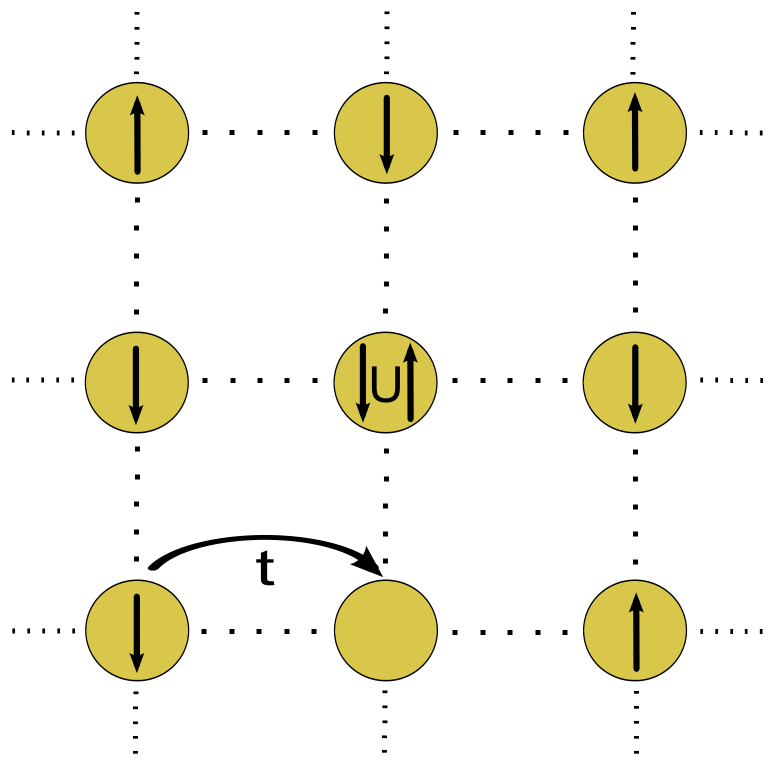
\includegraphics[width=0.29\linewidth]{fig/hubbard_model-scheme.png}
\caption{Schematization of the Hubbard model on a 2D square lattice. Electrons move to neighboring sites with a hopping $t$, and when two electrons are on the same site they feel a Coulomb repulsion $U$. Figure taken from \cite{thesis_dmft_graz}.}
\label{fig:hubbard_model-scheme}
\end{figure}

Putting together the ideas described in the last paragraph, we construct the hamiltonian of the Hubbard model in second quantization, given by
\begin{equation} \label{eq:hubbard-hamiltonian}
H = \eps_d \sum_{i, \s} n_{i\s} +  \sum_{\nn{i}{j}, \s} t_{ij} (c_{i\s}^\d c_{j\s} + \hc)
+ U \sum_{i} n_{i\up} n_{i\down}.
\end{equation}

The Hubbard model, although somewhat simple to define, does not have an analytic solution for general lattices. To grasp an understanding of this system, we must work with approximate solutions. Actually, Hubbard himself gave a simple approximate solution to the hamiltonian \ref{eq:hubbard-hamiltonian} in his seminal article, which is today known as ``Hubbard I Approximation'' (HIA). This solution uses the technique of retarted Green's functions described by Zubarev \cite{zubarev1960}, which we studied in the book \cite{bruus}.

While the HIA gives simple analytic expressions, it does not capture the metal-insulator phase transition that exists half-filling. In order to describe this transition, we went beyond and started learning the general method of Dynamical Mean-Field Theory (DMFT) \cite{georges1996}, which gives a reasonable treatment for the effects of electron correlations. In the next section we describe its details.

\subsection{DMFT} \label{sec:dmft}

Dynamical mean-field theory (DMFT) is a powerful method to treat strong correlations in materials. Its combination along with Density Functional Theory (DFT) makes a powerful computational tool to determine properties of real correlated electron materials \cite{hauleweb, haule_real_materials}.

DMFT is motivated by the establishment that it is exact in the limit of infinite lattice coordination $z \to \infty$, once there is a self-consistent mapping between the original hamiltonian onto a local impurity model \cite{thesis_dmft_graz}. In this limit, the self-energy $\displaystyle{\lim_{z \to \infty}\Sigma(\k,\omega) = \Sigma(\omega)}$ becomes \textit{local}, i.e., independent of the momentum $\k$.

Here we are going to illustrate DMFT in the context of the Hubbard model. In this case, the Hubbard hamiltonian is self-consistently mapped onto the Single Anderson Impurity Model (SIAM) \cite{impurity-solvers, georges1996}, where the impurity level, indexed by $d$, is coupled to an external bath:
\begin{equation} \label{eq:anderson-hamiltonian}
H_{\text{SIAM}} = \underbrace{U n_{d\up} n_{d\down} + \eps_d \sum_{\s} n_{d\s}}_{H_{\text{imp}}}
+ \underbrace{\sum_{\k,\s} (t_\k c_{d\s}^\d c_{k\s} + \hc)}_{H_{\text{coup}}}
+ \underbrace{\sum_{\k,\s} \eps_\k c_{\k\s}^\d c_{\k\s}}_{H_{\text{bath}}}.
\end{equation}

In equation \ref{eq:anderson-hamiltonian}, $H_{\text{bath}}$ is the hamiltonian of the bath, $H_{\text{coup}}$ is the coupling between the bath and the single impurity $d$, and $H_{\text{imp}}$ is the hamiltonian of the impurity. $H_{\text{imp}}$, anologously with the Hubbard hamiltonian in equation \ref{eq:hubbard-hamiltonian}, has an interaction $U$ when two electrons are on the same site.

The SIAM is an impurity problem, which is relatively easier to solve numerically than the Hubbard model, that consist of a lattice problem. There are several methods, known as impurity solvers, available in the literature that attempt to solve systems such as the SIAM. Reference \cite{impurity-solvers} gives an overview and a benchmark of some impurity solvers.

By solving an impurity problem, we actually mean determining the retarded Green's function of the impurity site $G_{\text{imp}}(\omega)$, because its knowledge allows us compute the spectral function $\displaystyle{\rho(\omega) = - \frac{1}{\pi} \Im{G_{\text{imp}}(\omega)}}$ \cite{bruus} and a manifold of important observables related to quantum transport \cite{pedagogical-gfs}.

\begin{figure}[H]
\centering
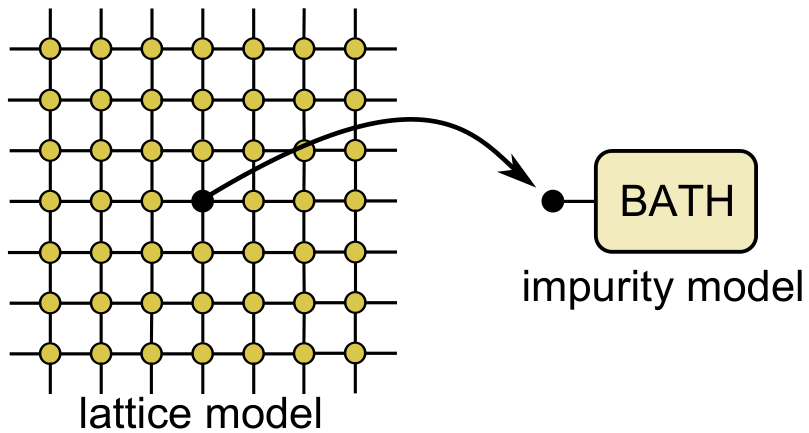
\includegraphics[width=0.6\linewidth]{fig/dmft-mapping}
\caption{Schematization of the mapping between the lattice problem and a single impurity coupled to an effective bath. Figure taken from \cite{thesis_dmft_graz}.}
\label{fig:dmft-mapping}
\end{figure}

Having in mind this map onto an impurity problem, the DMFT scheme is based on the approximation
\begin{equation} \label{eq:dmft-approx}
\Sigma(\k, \omega) \approx \Sigma(\omega),
\end{equation}
where we assume that the self-energy is approximately independent of $\k$, guided by the fact that this is an equality in the limit where $z \to \infty$ and corresponds to localized solutions. Along with this approximation, the self-consistency tells us that the local lattice Green's function $G_{\text{loc}}(\omega)$ coincides with the impurity model's Green function $G_{\text{imp}}(\omega)$, and this translates into a convergence criterion for the DMFT algorithm.

Hence, using equation \ref{eq:dmft-approx}, the local lattice Green's function in the continuum limit can be written as
\begin{equation} \label{eq:Gf-local}
G_{\text{loc}}(\omega) = \sum_{\k} \frac{1}{\omega-\eps_\k-\Sigma(\k, \omega)} \approx
\int \dd{\eps} \frac{\rho_0(\eps)}{\omega - \eps - \Sigma(\omega)},
\end{equation}
where $\rho_0(\eps)$ is the non-interacting density of states (DOS) and depends only on the considered lattice structure, defined by
\begin{equation} \label{eq:non-interacting-DOS}
\rho_0(\eps) = \sum_{\k} \delta(\eps-\eps_\k).
\end{equation}

In essence, the general DMFT algorithm works as follows. Firstly, we start with an initial guess for the self-energy $\Sigma(\omega)$ and compute $G_{\text{loc}}(\omega)$ by equation \ref{eq:Gf-local}. On the other hand, the impurity solver (NCA) takes the bath hybridization function $\Delta(\omega)$, given by
\begin{equation} \label{eq:hybridization-func}
\Delta(\omega) = \omega - \eps_d - G_{\text{loc}}^{-1}(\omega) - \Sigma(\omega),
\end{equation}
and returns $G_{\text{imp}}(\omega)$ by solving the SIAM. We compare $G_{\text{loc}}$ and $G_{\text{imp}}$ with some convergence criterion and, if this criterion is not satisfied, we update the self-energy by
\begin{equation} \label{eq:self-energy-update}
\Sigma(\omega) = \omega - \eps_d - G_{\text{imp}}^{-1}(\omega).
\end{equation}

Using a basic property of the spectral function $\rho(\omega)$, the filling $n$ is given by \cite{bruus}
\begin{equation} \label{eq:filling}
n = \int_{-\infty}^{\infty} f(\omega, T) \rho(\omega) \dd{\omega},
\end{equation}
where $f(\omega, T) = (e^{\omega/k_B T} + 1)^{-1}$ is the Fermi-Dirac distribution at temperature $T$.

\subsection{Bethe lattice} \label{sec:bethe}

The Bethe lattice is an infinite lattice where each site has $z$ neighbors and any two sites are connected by a unique shortest path. Figure \ref{fig:bethe-lattice} represents a Bethe lattice in the case where $z = 4$.
\begin{figure}[H]
\centering
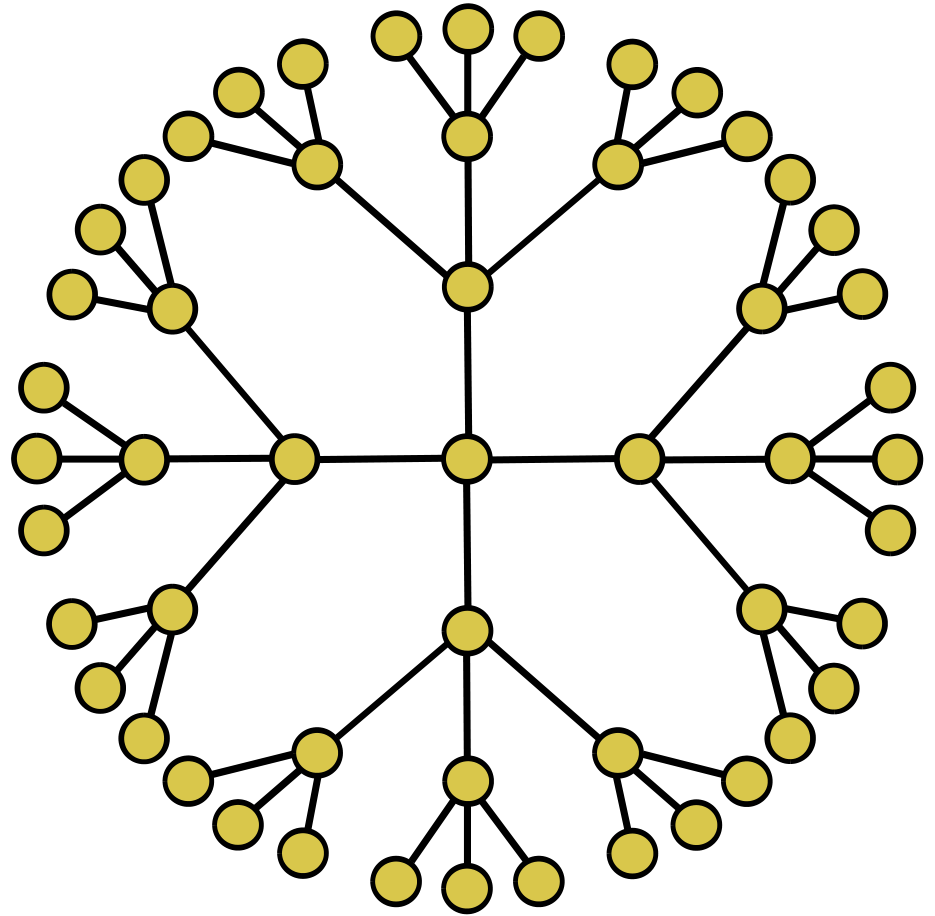
\includegraphics[width=0.4\linewidth]{fig/bethe-lattice.png}
\caption{Schematization of the Bethe lattice with coordination number $z = 4$. The lattice is actually infinite and all sites equivalent. Figure taken from \cite{thesis_dmft_graz}.}
\label{fig:bethe-lattice}
\end{figure}

In our DMFT work, we focused on the special case of the Bethe lattice with infinite coordination $z\to\infty$, which was extensively studied in the literature \cite{georges1996, thesis_dmft_graz} and serves as a benchmark for the DMFT algorithm because the expressions simplify a lot in this setting. But the Hubbard hamiltonian in equation \ref{eq:hubbard-hamiltonian} only makes sense for a Bethe lattice with $z\to\infty$ if the hopping amplitude is renormalized as \cite{thesis_bruno}
\begin{equation} \label{eq:hopping-renormalization}
t = \frac{t_*}{\sqrt{z}},
\end{equation}
where $t_*$ is the renormalized hopping parameter.

The non-interacting DOS $\rho(\eps)$ for the Bethe lattice has a semicircular form \cite{georges1996}
\begin{equation} \label{eq:bethe-dos}
\rho_0(\eps) = \frac{2}{\pi D} \sqrt{1-\qty(\frac{\omega}{D})^2},
\end{equation}
where $D = 2t^*$ is the half-bandwidth. We use $D = 1$ as energy unit, such that $t_* = 1/2$.


Using equation \ref{eq:bethe-dos} and integrating equation \ref{eq:Gf-local}, one can obtain the relation \cite{thesis_bruno}
\begin{equation} \label{eq:simple-hybridization-bethe}
\Delta(\omega) = t_*^2 \, G_{\text{imp}}(\omega),
\end{equation}
which simplifies a lot the DMFT loop since the update of the hybridization function is trivial and it can be directly inserted in the new iteration of the impurity solver.

\subsection{Impurity Solver} \label{sec:impurity-solver}

As our main objective was to establish a working code for DMFT and to probe the metal-insulator transition for the Hubbard model, we chose to use the Non-Crossing Approximation (NCA) impurity solver. As can be seen in Table 1 of \cite{impurity-solvers}, the NCA has a low computational-cost while still giving reasonable qualitative results, but it is important to keep in mind that it does not return accurate quantitative values for critical interactions $U_{c1}$, $U_{c2}$ and Kondo temperature $T_{\text{K}}$ \cite{haule_real_materials, vildosola2015}. The NCA method also has the advantage of quickly accessing a versatile range of temperatures.

The NCA algorithm is very lengthy to describe but all its details can be found in Section 2.2 of \cite{thesis_bruno}. For our work, we used the NCA code developed by Kristjan Haule available on the website \cite{hauleweb}. The code takes as input the bath hybridization function $\Delta(\omega)$ and returns the Green's function $G_{\text{imp}}(\omega)$. Because of the simplified DMFT equation \ref{eq:simple-hybridization-bethe} for the Bethe lattice, the DMFT loop is reduced to basically applying the impurity solver and updating the hybridization function until convergence is reached. In the next section (Sec. \ref{sec:results}) we present the results obtained with our settings.

\subsection{Results} \label{sec:results}

Firstly, we explored the standard setting in the literature \cite{georges1996}, that is the case of $\eps_d = U/2$, where the system is always at half-filling ($n=1$) because the hamiltonian \ref{eq:hubbard-hamiltonian} is particle-hole symmetric (PHS). When the temperature is low enough such that a coexistence region exists, there are two values of critical interaction strength $U$ where the system experiences a phase transition. When one starts from an Mott insulating solution at large $U$ and then decreases it, the system reaches a critical value $U_{c_1}$ for which it becomes metallic. On the other hand, when starting from a metallic solution at low $U$ and increasing it, the system reaches another critical value $U_{c2} > U_{c1}$, for which it becomes an insulator. To characterize these two phases, we use the spectral density $\rho(\omega = 0)$ and the filling $n$. It is known that the Mott insulating phase only exists at half-filling ($n=1$) \cite{georges1996} and, from linear response theory, that the spectral function at the Fermi energy (zero) gives a good criterion if the system is metallic ($\rho(\omega=0) > 0$) or insulating ($\rho(\omega=0) = 0$).

In Figure \ref{fig:triangle-mu050} we make a color plot of the average $\rho_{\text{mean}} = (\rho_{\text{metal}}(0) + \rho_{\text{insul}}(0))/2$ as a function of $U \times T$, where the ``metal'' and ``insul'' labels mean starting with a metallic (low $U$) or insulating (high $U$) solution. The blue region, where $\rho_{\text{mean}} = 0$, corresponds to the insulating phase and the red region $\rho_{\text{mean}}$ is very high corresponds to the metallic phase. We see that the colors change abruptally (red $\to$ green $\to$ blue) for $T < T_c \approx 0.008$ and smoothly for $T > T_c$. This means a coexistence region (the triangle in green) for $T < T_c$ and a crossover region for $T > T_c$.

\begin{figure}[H]
\centering
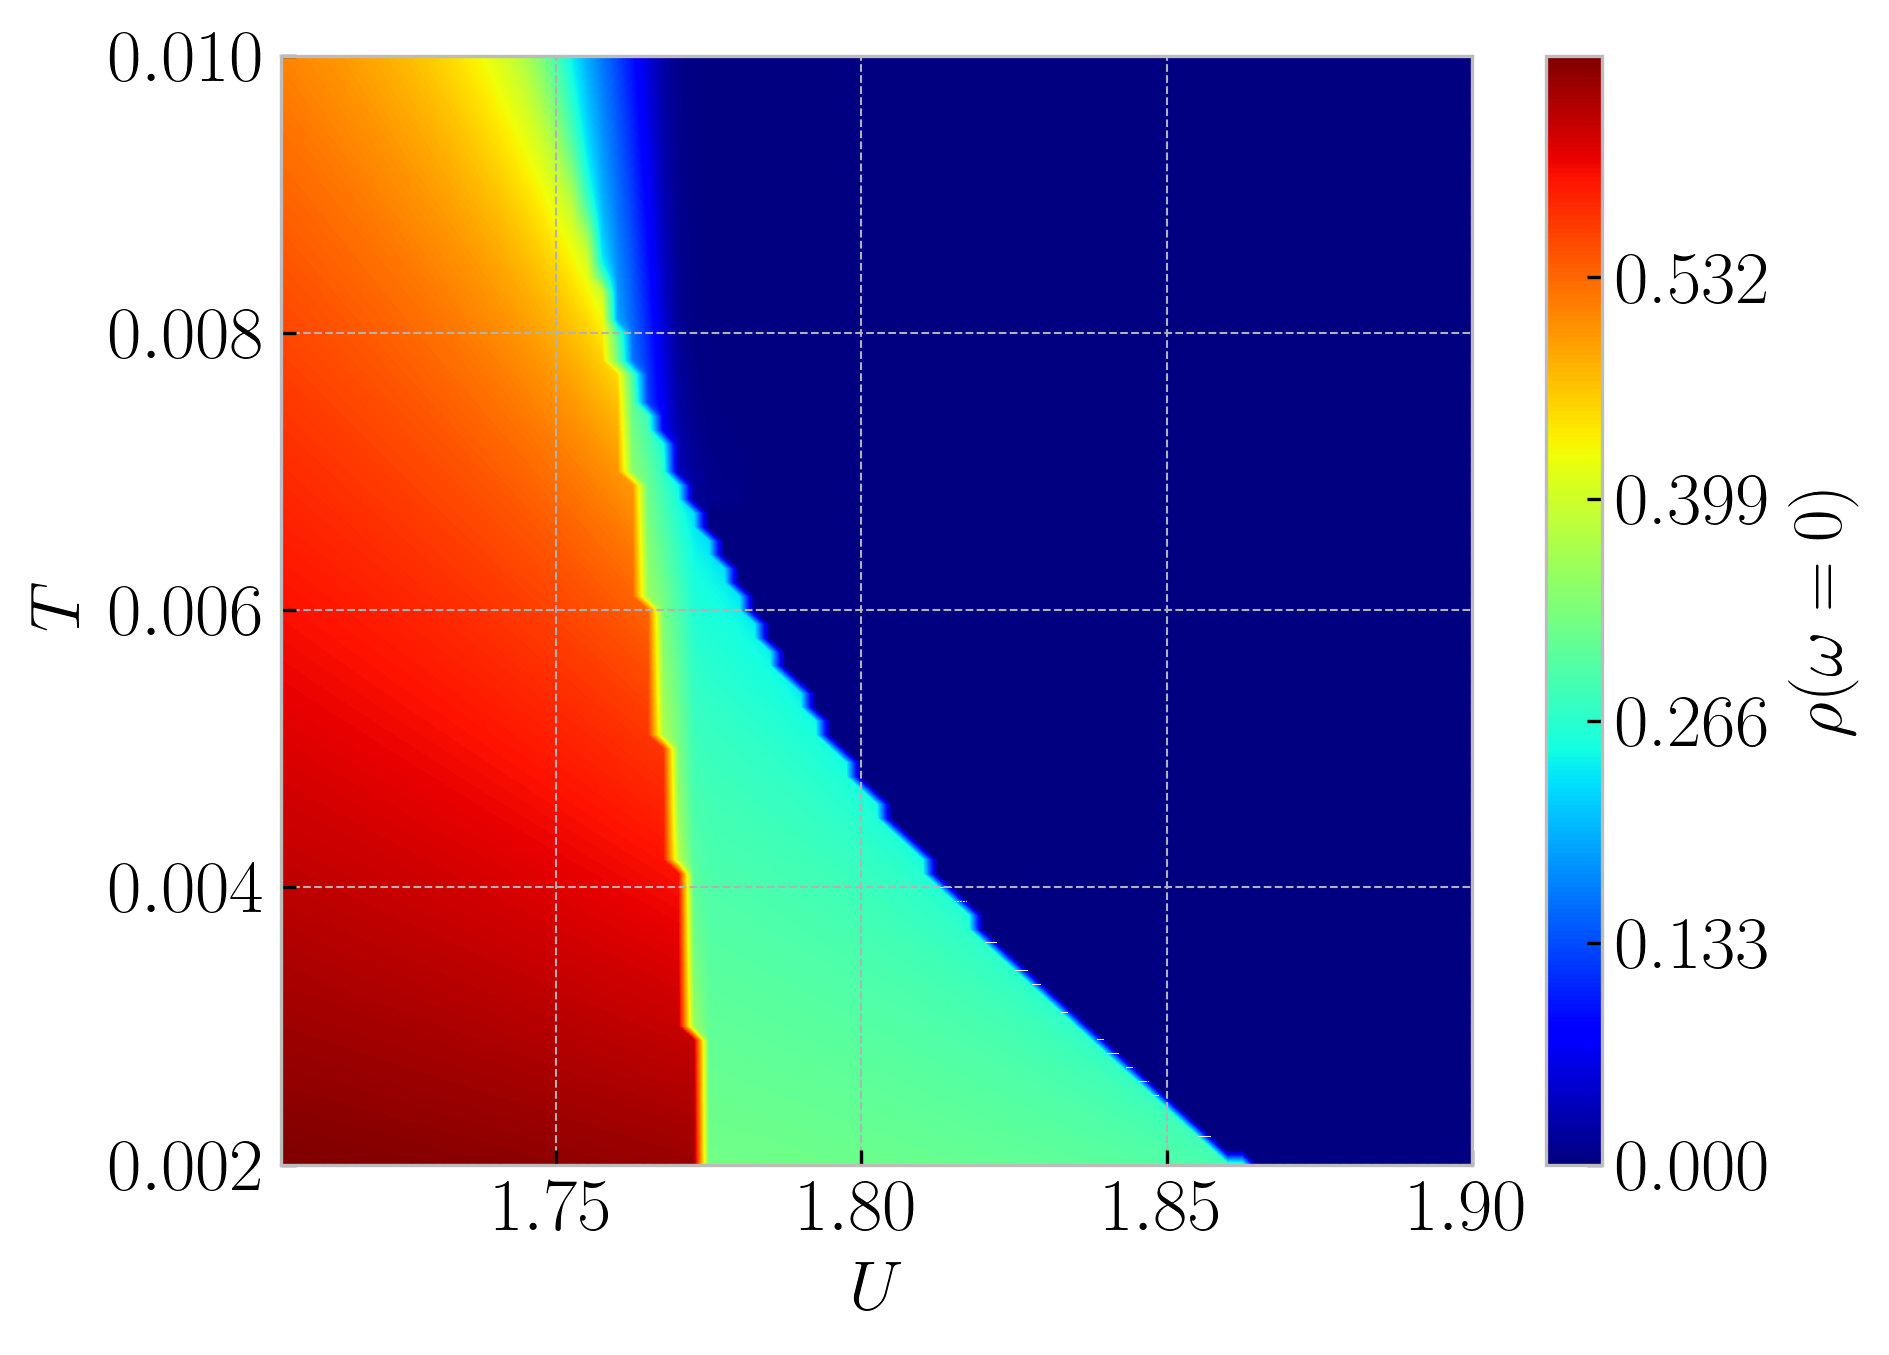
\includegraphics[width=0.41\textwidth]{fig/dmft/triangle-w0-mu050.png}
\caption{Phase diagram  $U \times T$ for the Hubbard model at $\epsilon_d=U/2$ obtained with the DMFT-NCA approximation. The color code shows the average $\rho_{\text{mean}}$. The coexistence region is marked in green.}
\label{fig:triangle-mu050}
\end{figure}

Figure \ref{fig:mu045} shows an analogous $U \times T$ phase diagram, but for $\eps_d = 0.45 \, U$, where the system is not necessarily at half-filling. Because of this, we also plot the filling $n_{\text{mean}} = (n_{\text{metal}} + n_{\text{insul}}(0))/2$, along with $\rho_{\text{mean}}$. We clearly see that both plots in Figure \ref{fig:mu045} show a similar phase diagram pattern. One thing to notice is that the coexistence triangular region is narrower than the case PHS case in Figure \ref{fig:triangle-mu050}. Mesmerized by this, we went on to examine the behavior of the coexistence region for different values of $\eps_d/U$.

\begin{figure}[H]
\centering
\begin{subfigure}{.40\textwidth}
  \centering
  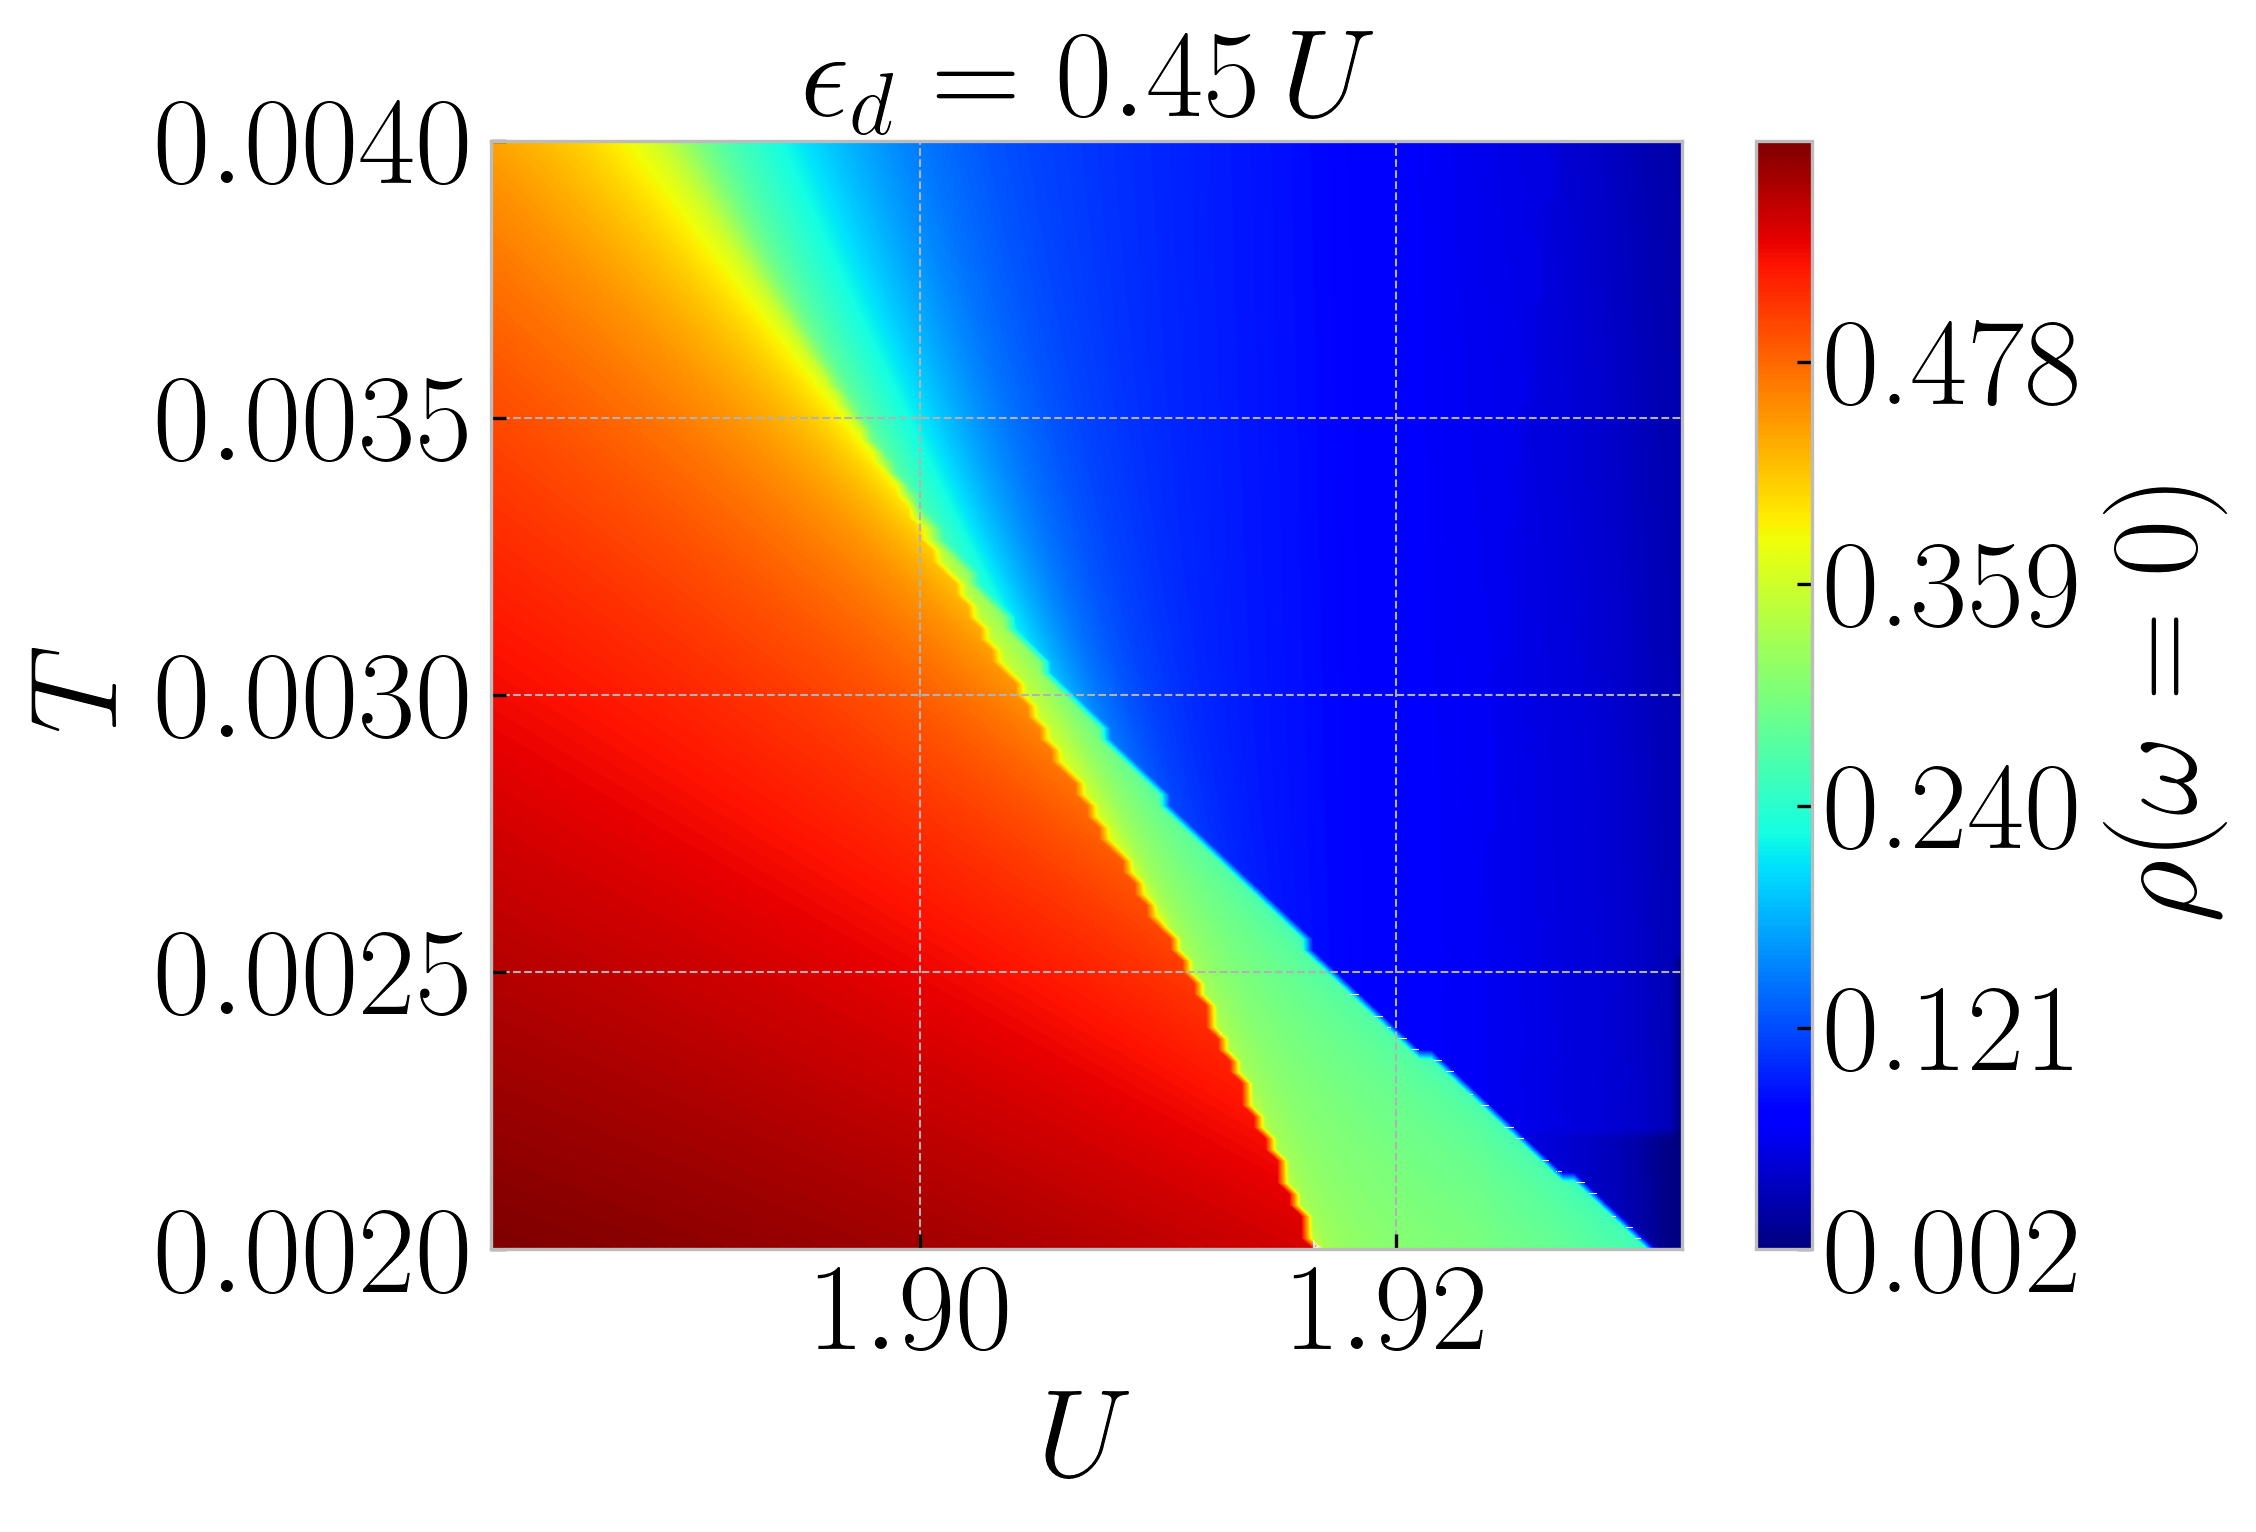
\includegraphics[width=\linewidth]{fig/dmft/mean2_0-mu045.png}
  \caption{}
  \label{fig:mu045-rho0}
\end{subfigure}%
\hfill
\begin{subfigure}{.40\textwidth}
  \centering
  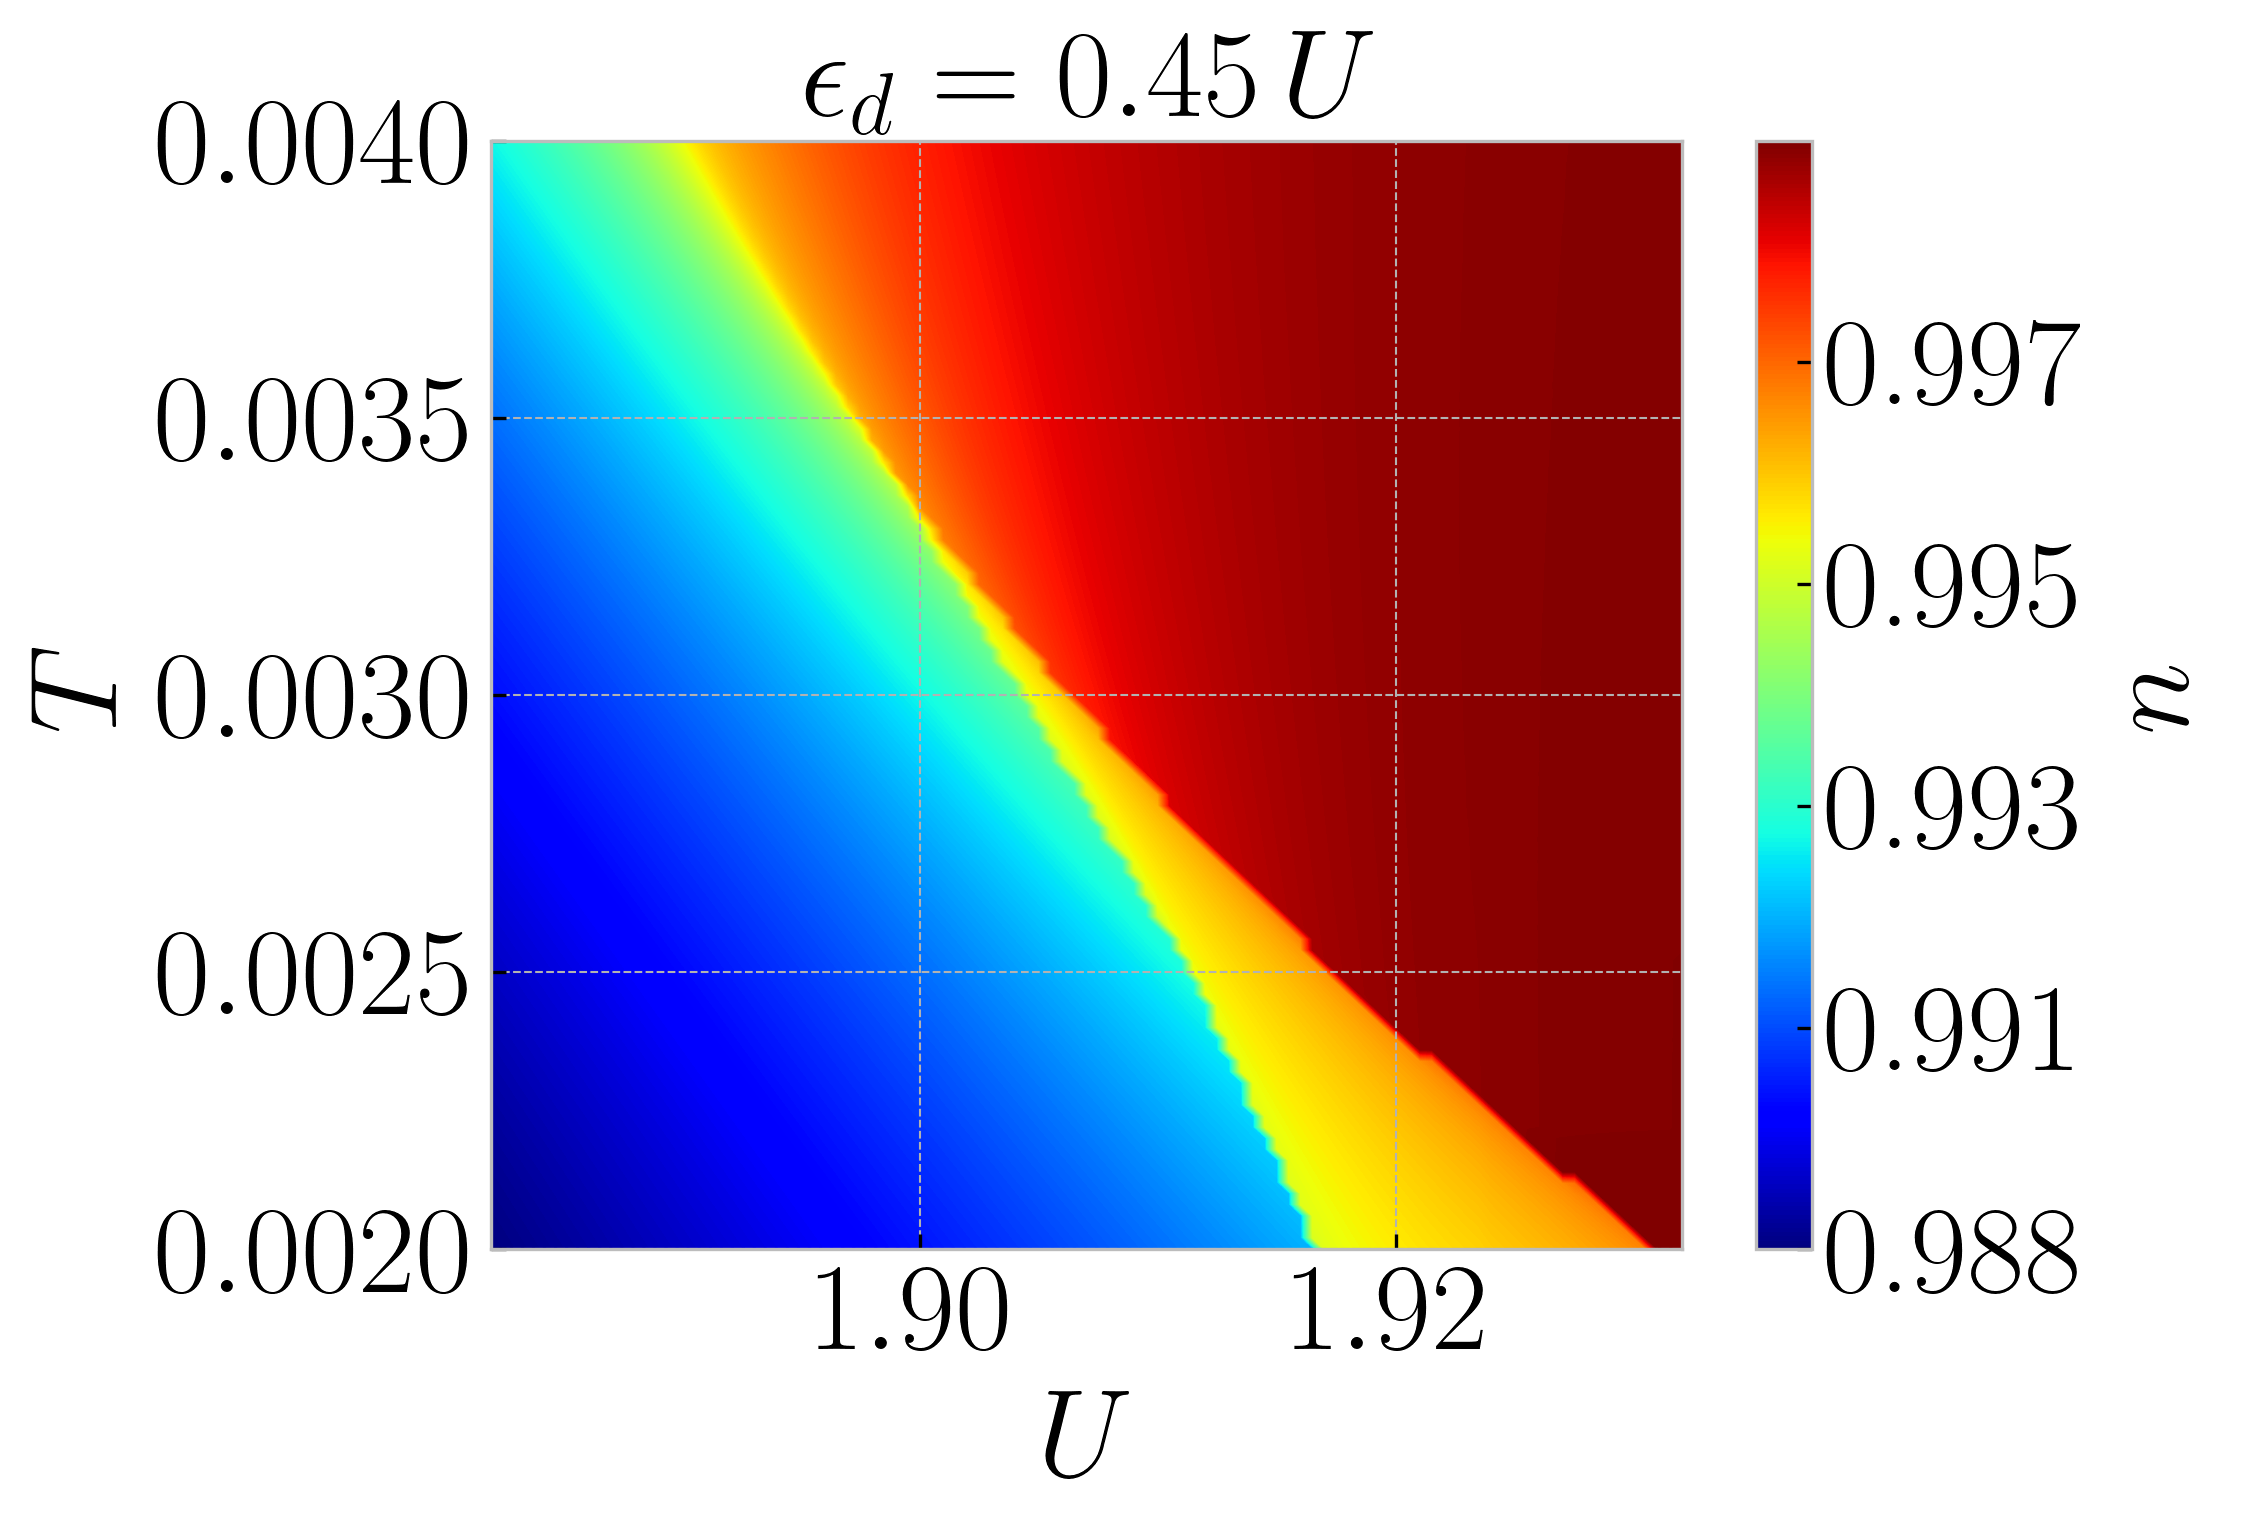
\includegraphics[width=\linewidth]{fig/dmft/mean2_n-mu045.png}
  \caption{}
  \label{fig:mu045-n}
\end{subfigure}
\caption{Phase diagrams $U \times T$ for on-site energy $\eps_d = 0.45 \, U$, which show the $\rho_{\text{mean}}$ in (a) and $n_{\text{mean}}$ in (b).}
\label{fig:mu045}
\end{figure}

In Figure \ref{fig:Diagram_Drho_U_T_coex} we show $U \times T$ phase diagrams of $\rho_{\text{mean}}$, which enable us to visualize that the coexistence region (in green) grows as $\eps_d$ approaches $U/2$.



\begin{figure}[H]
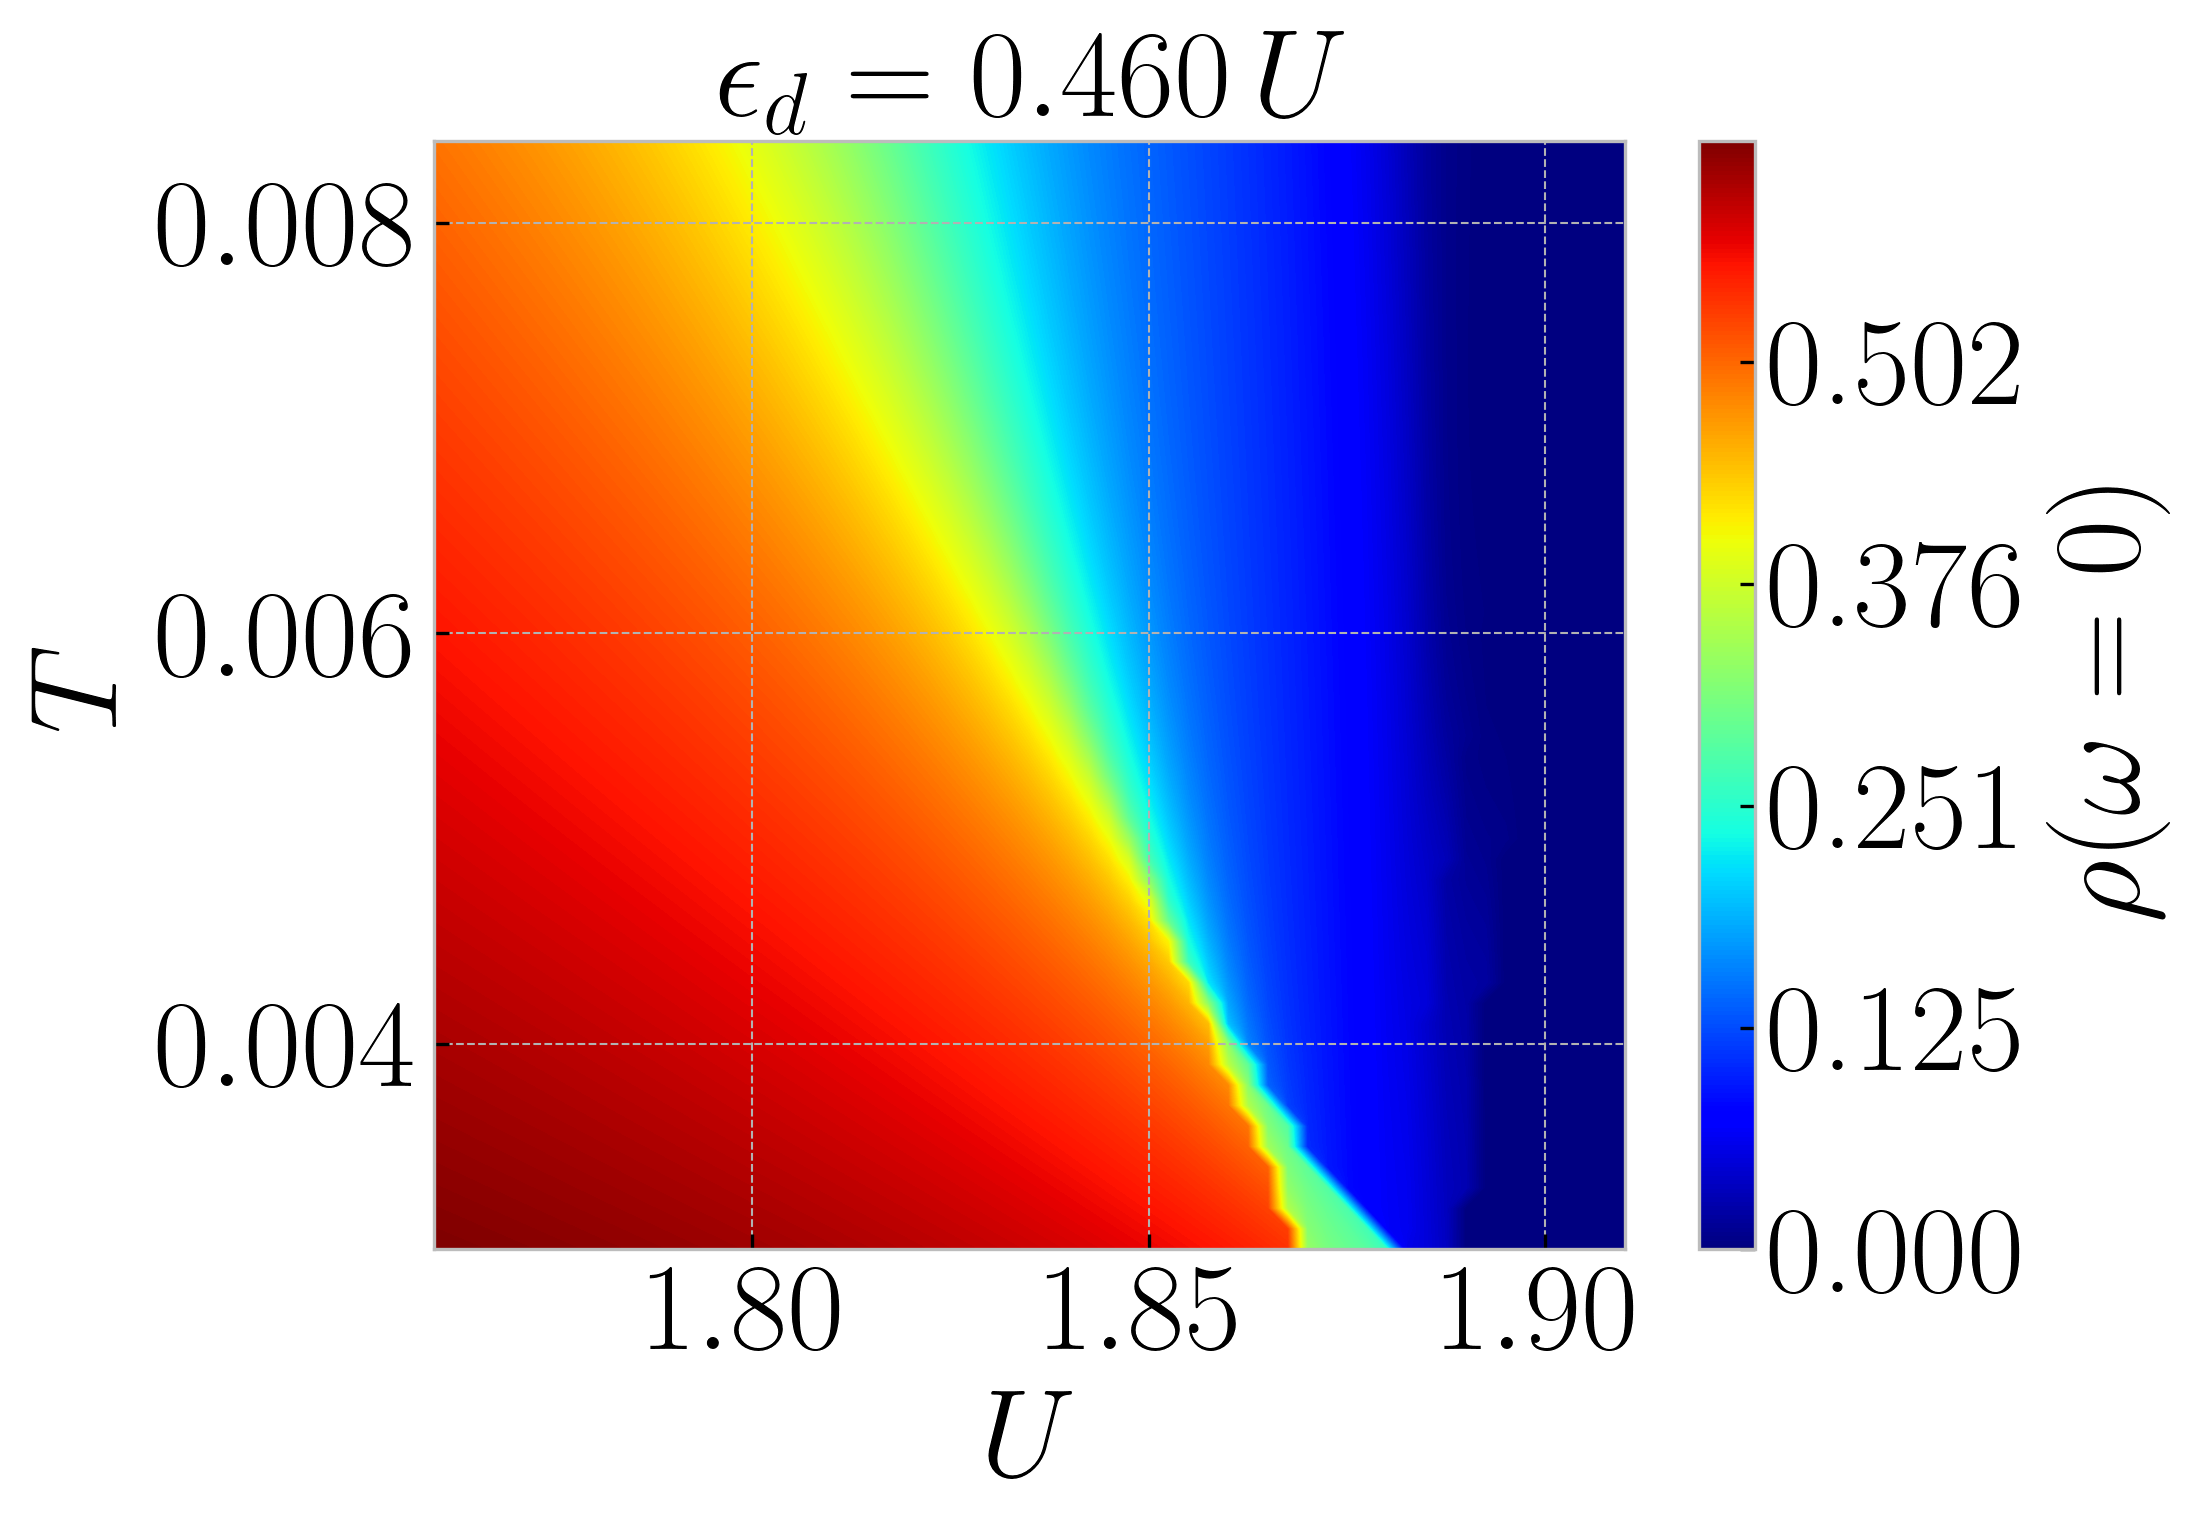
\includegraphics[width=0.42\textwidth]{fig/dmft/coex_mean-df_0-mu=0.460.png}
\hfill
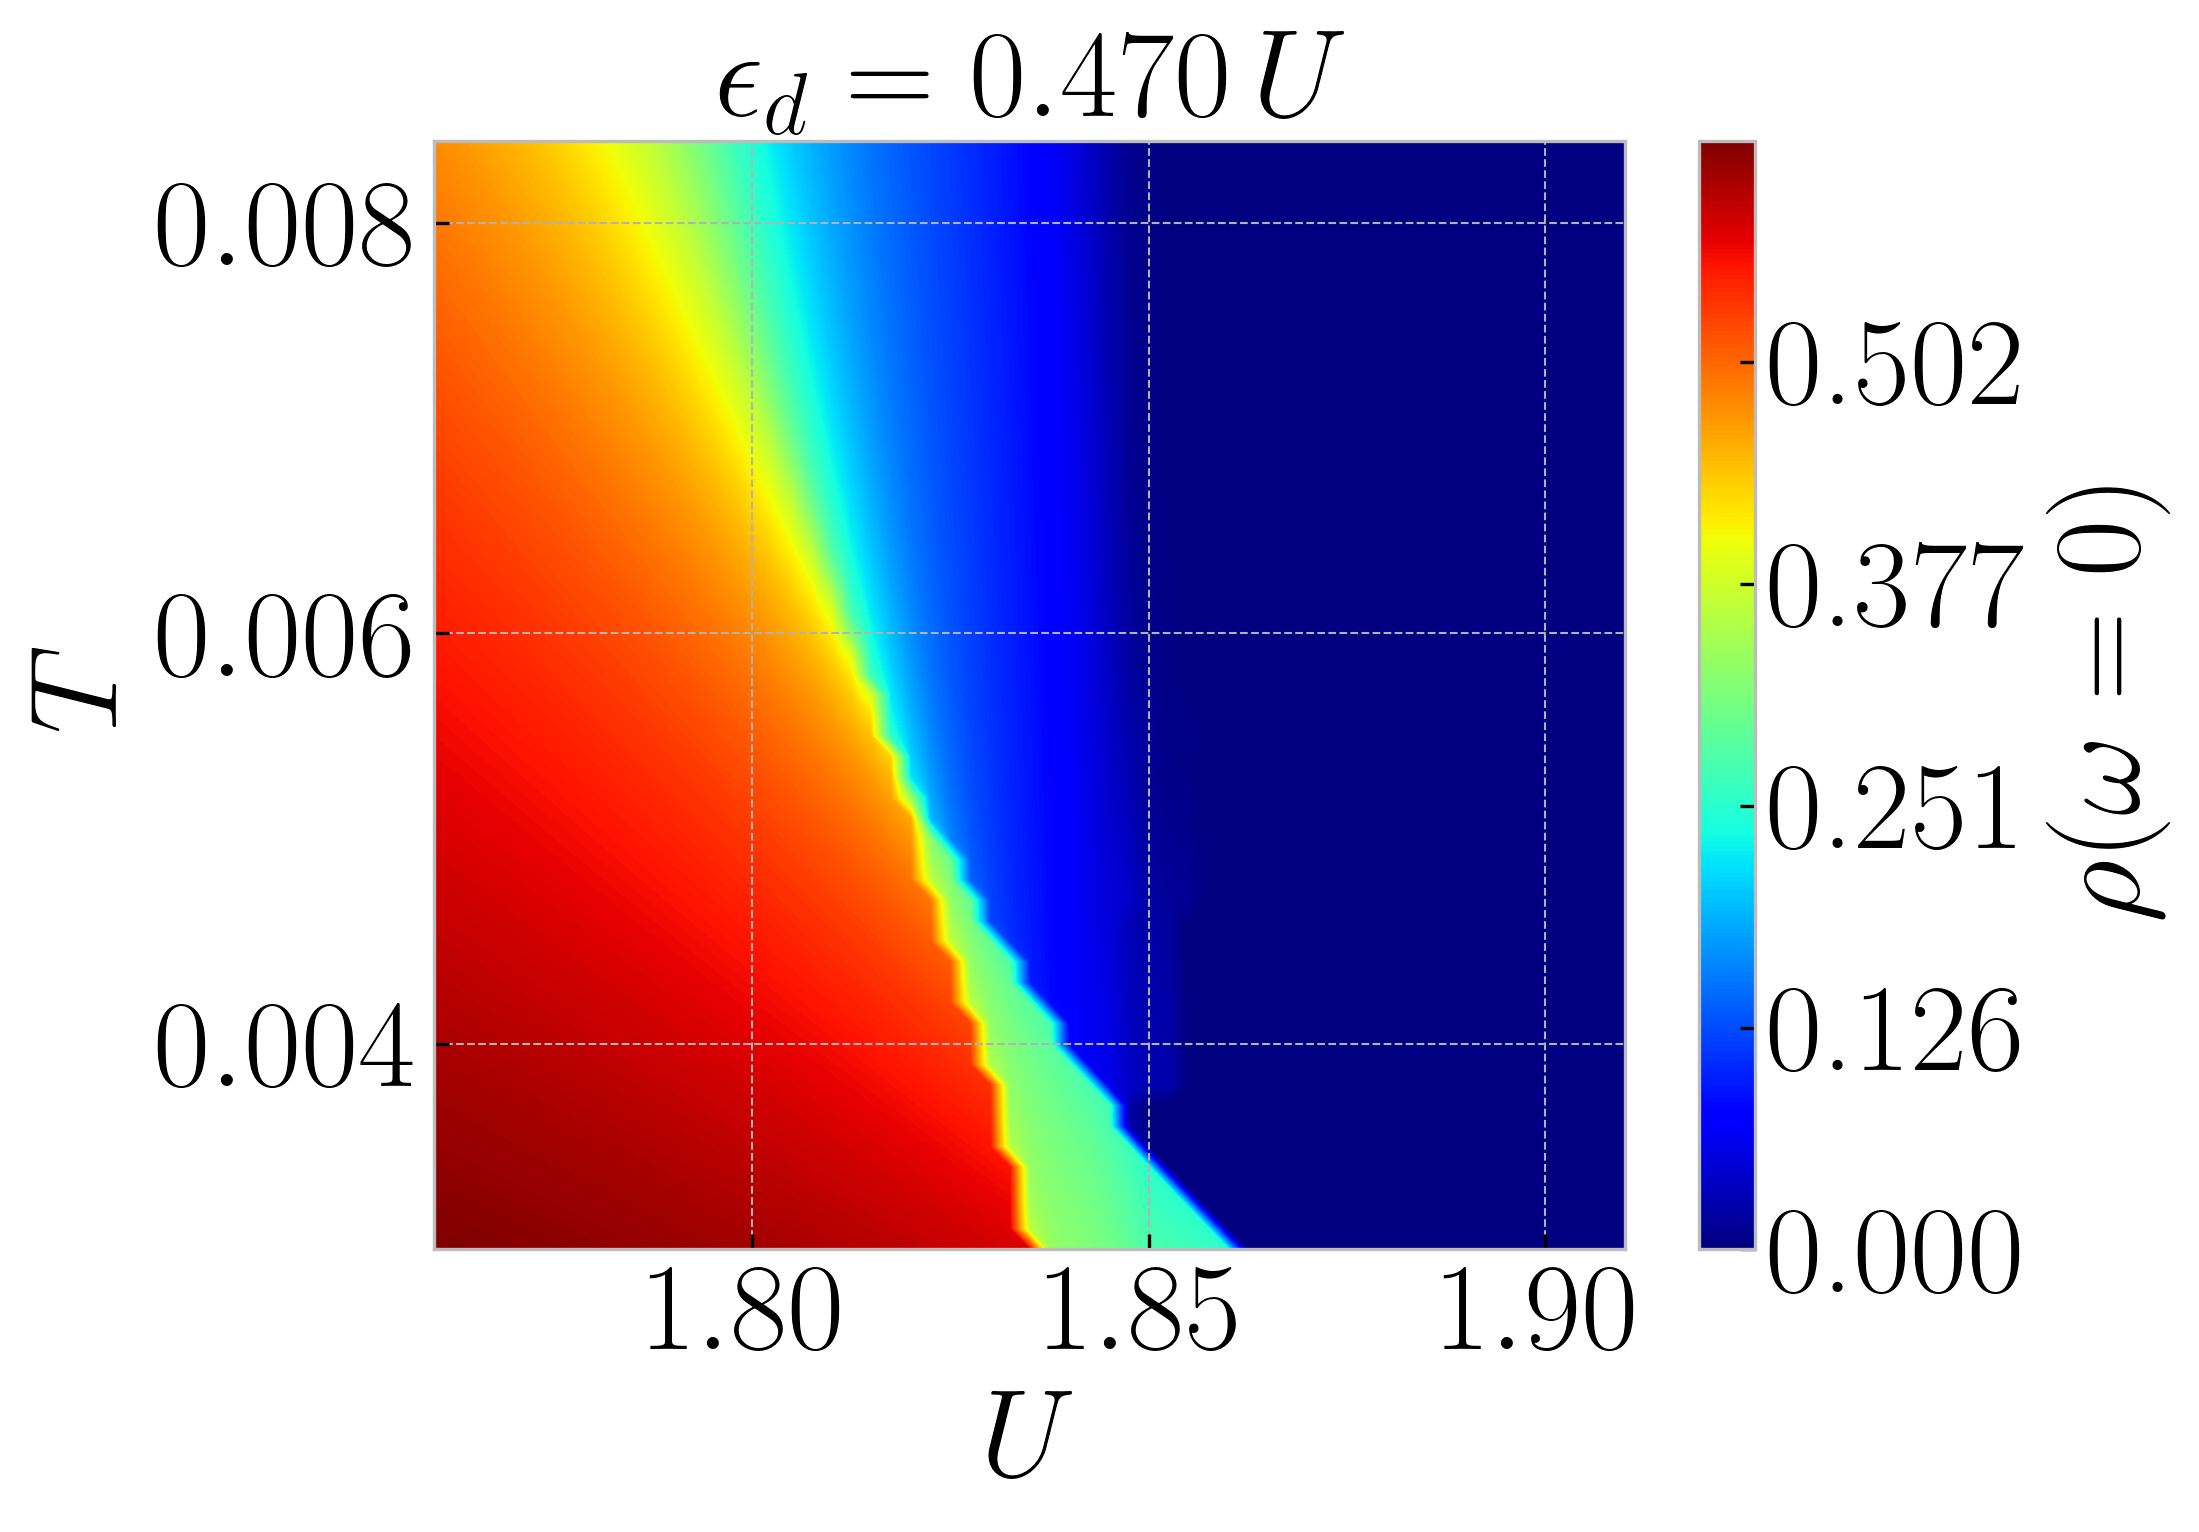
\includegraphics[width=0.42\textwidth]{fig/dmft/coex_mean-df_0-mu=0.470.png}
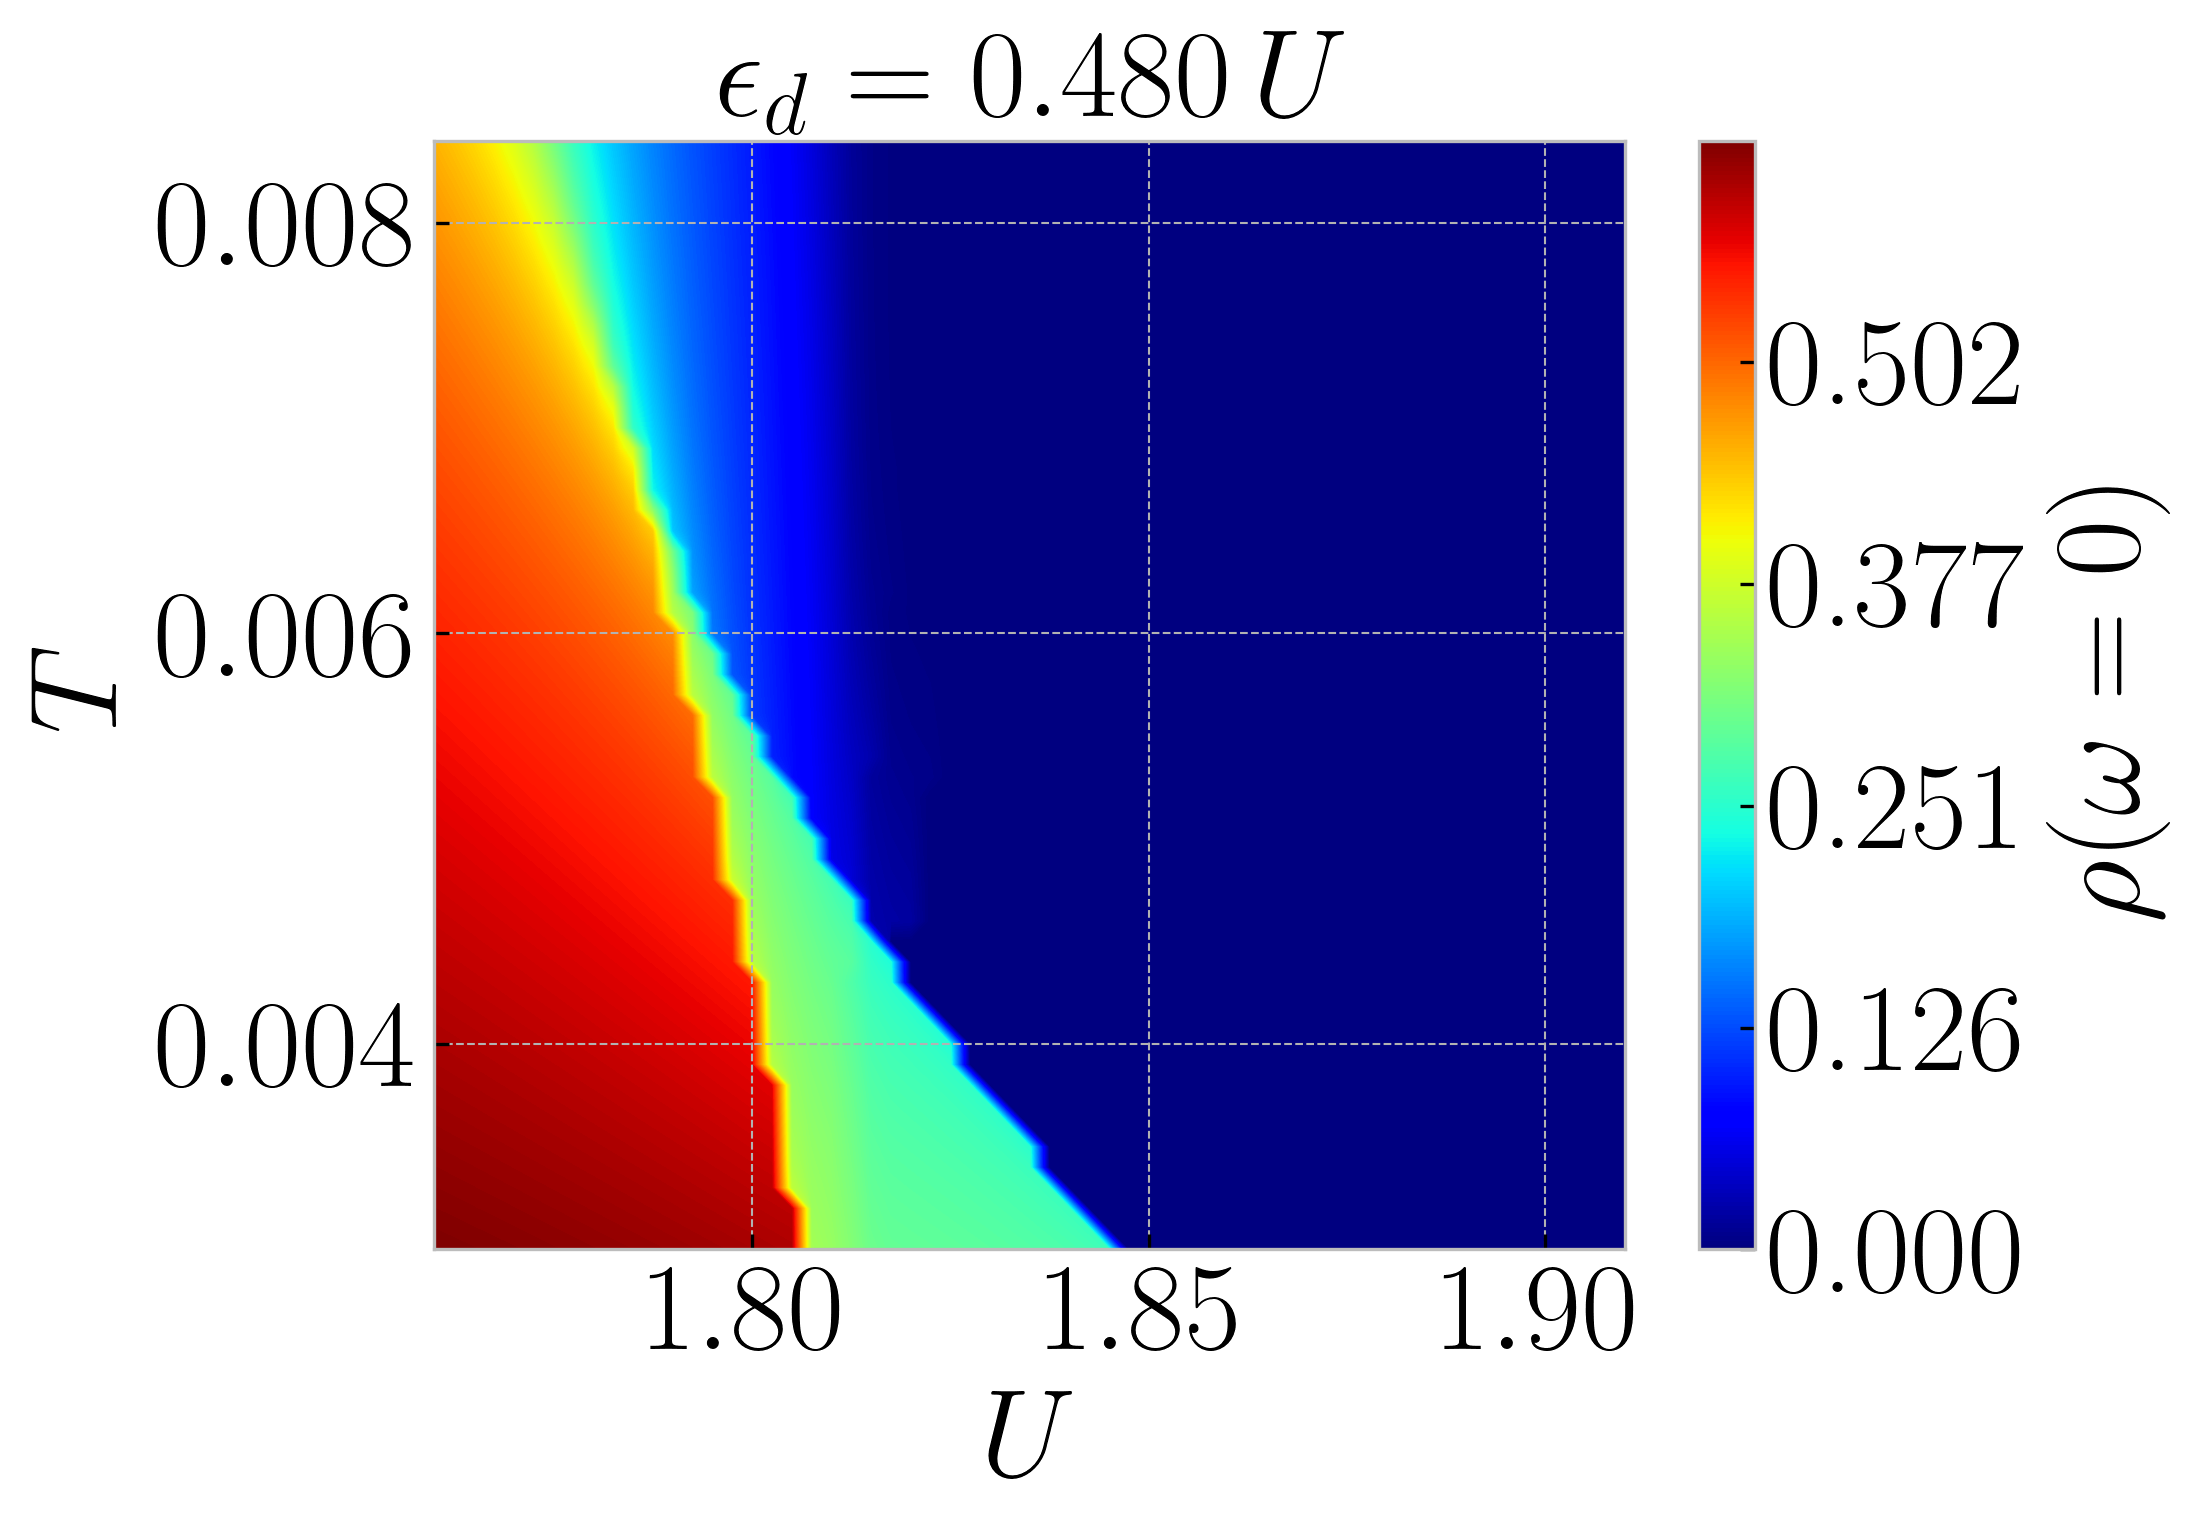
\includegraphics[width=0.42\textwidth]{fig/dmft/coex_mean-df_0-mu=0.480.png}
\hfill
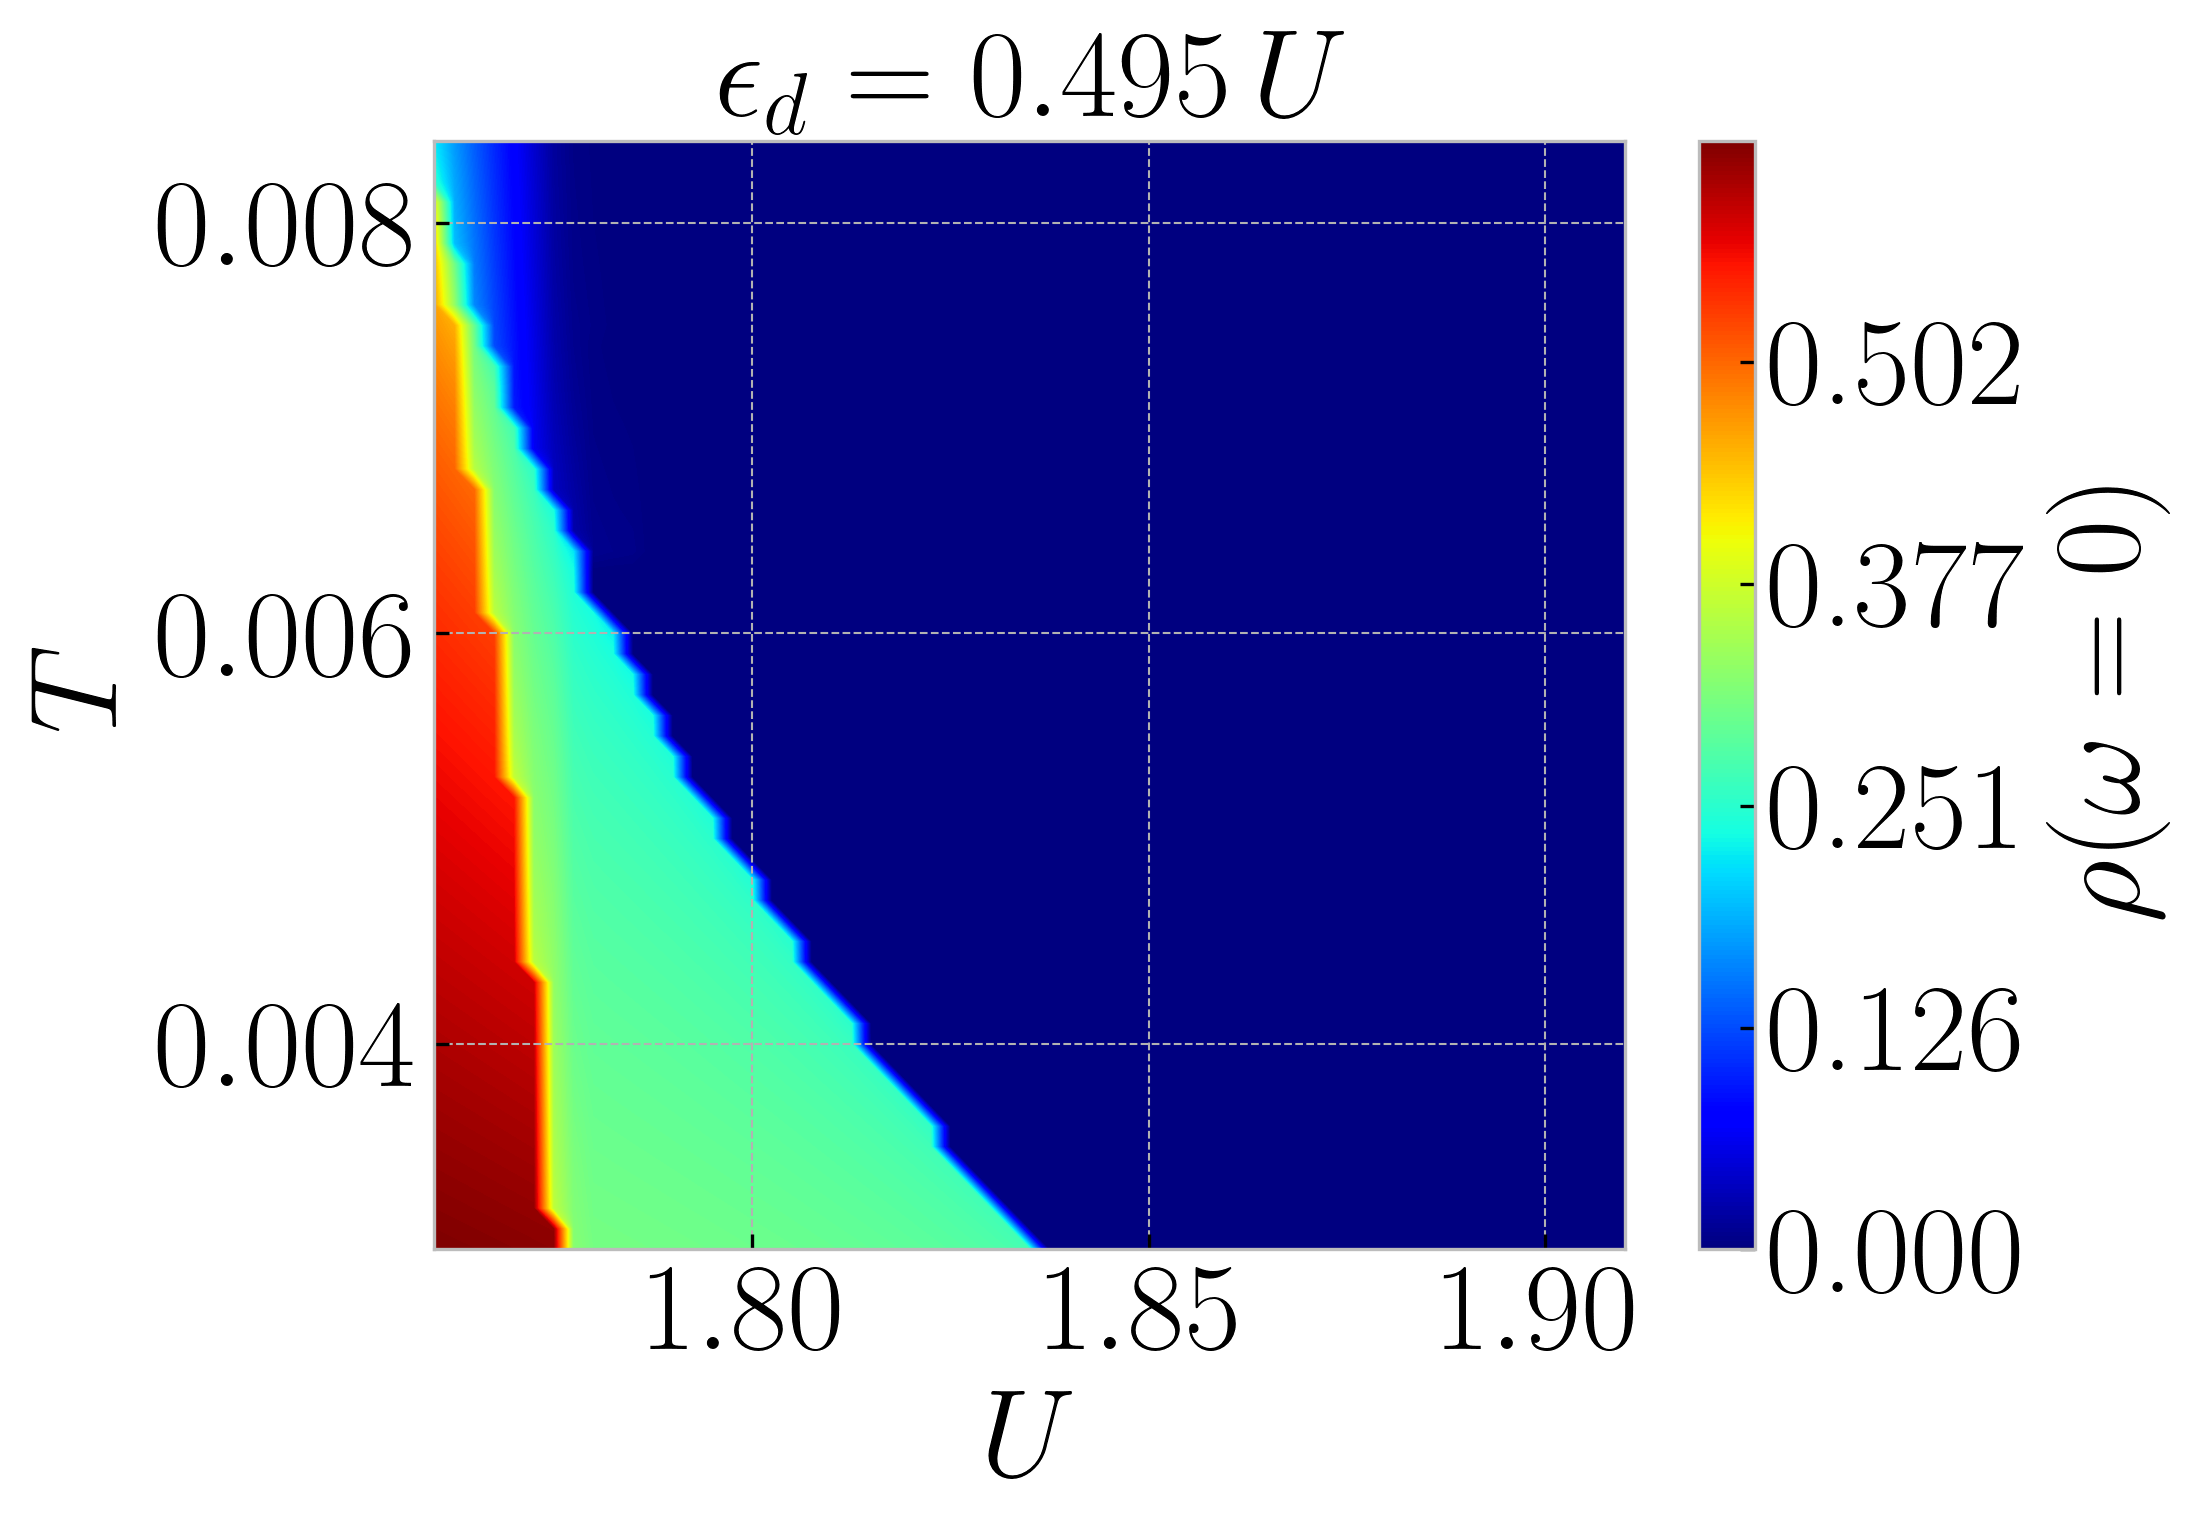
\includegraphics[width=0.42\textwidth]{fig/dmft/coex_mean-df_0-mu=0.495.png}
\caption{Phase diagrams $U \times T$ for on-site energies $\eps_d/U = 0.46$, $0.47$, $0.48$, $0.495$.}
\label{fig:Diagram_Drho_U_T_coex}
\end{figure}



\begin{figure}[H]
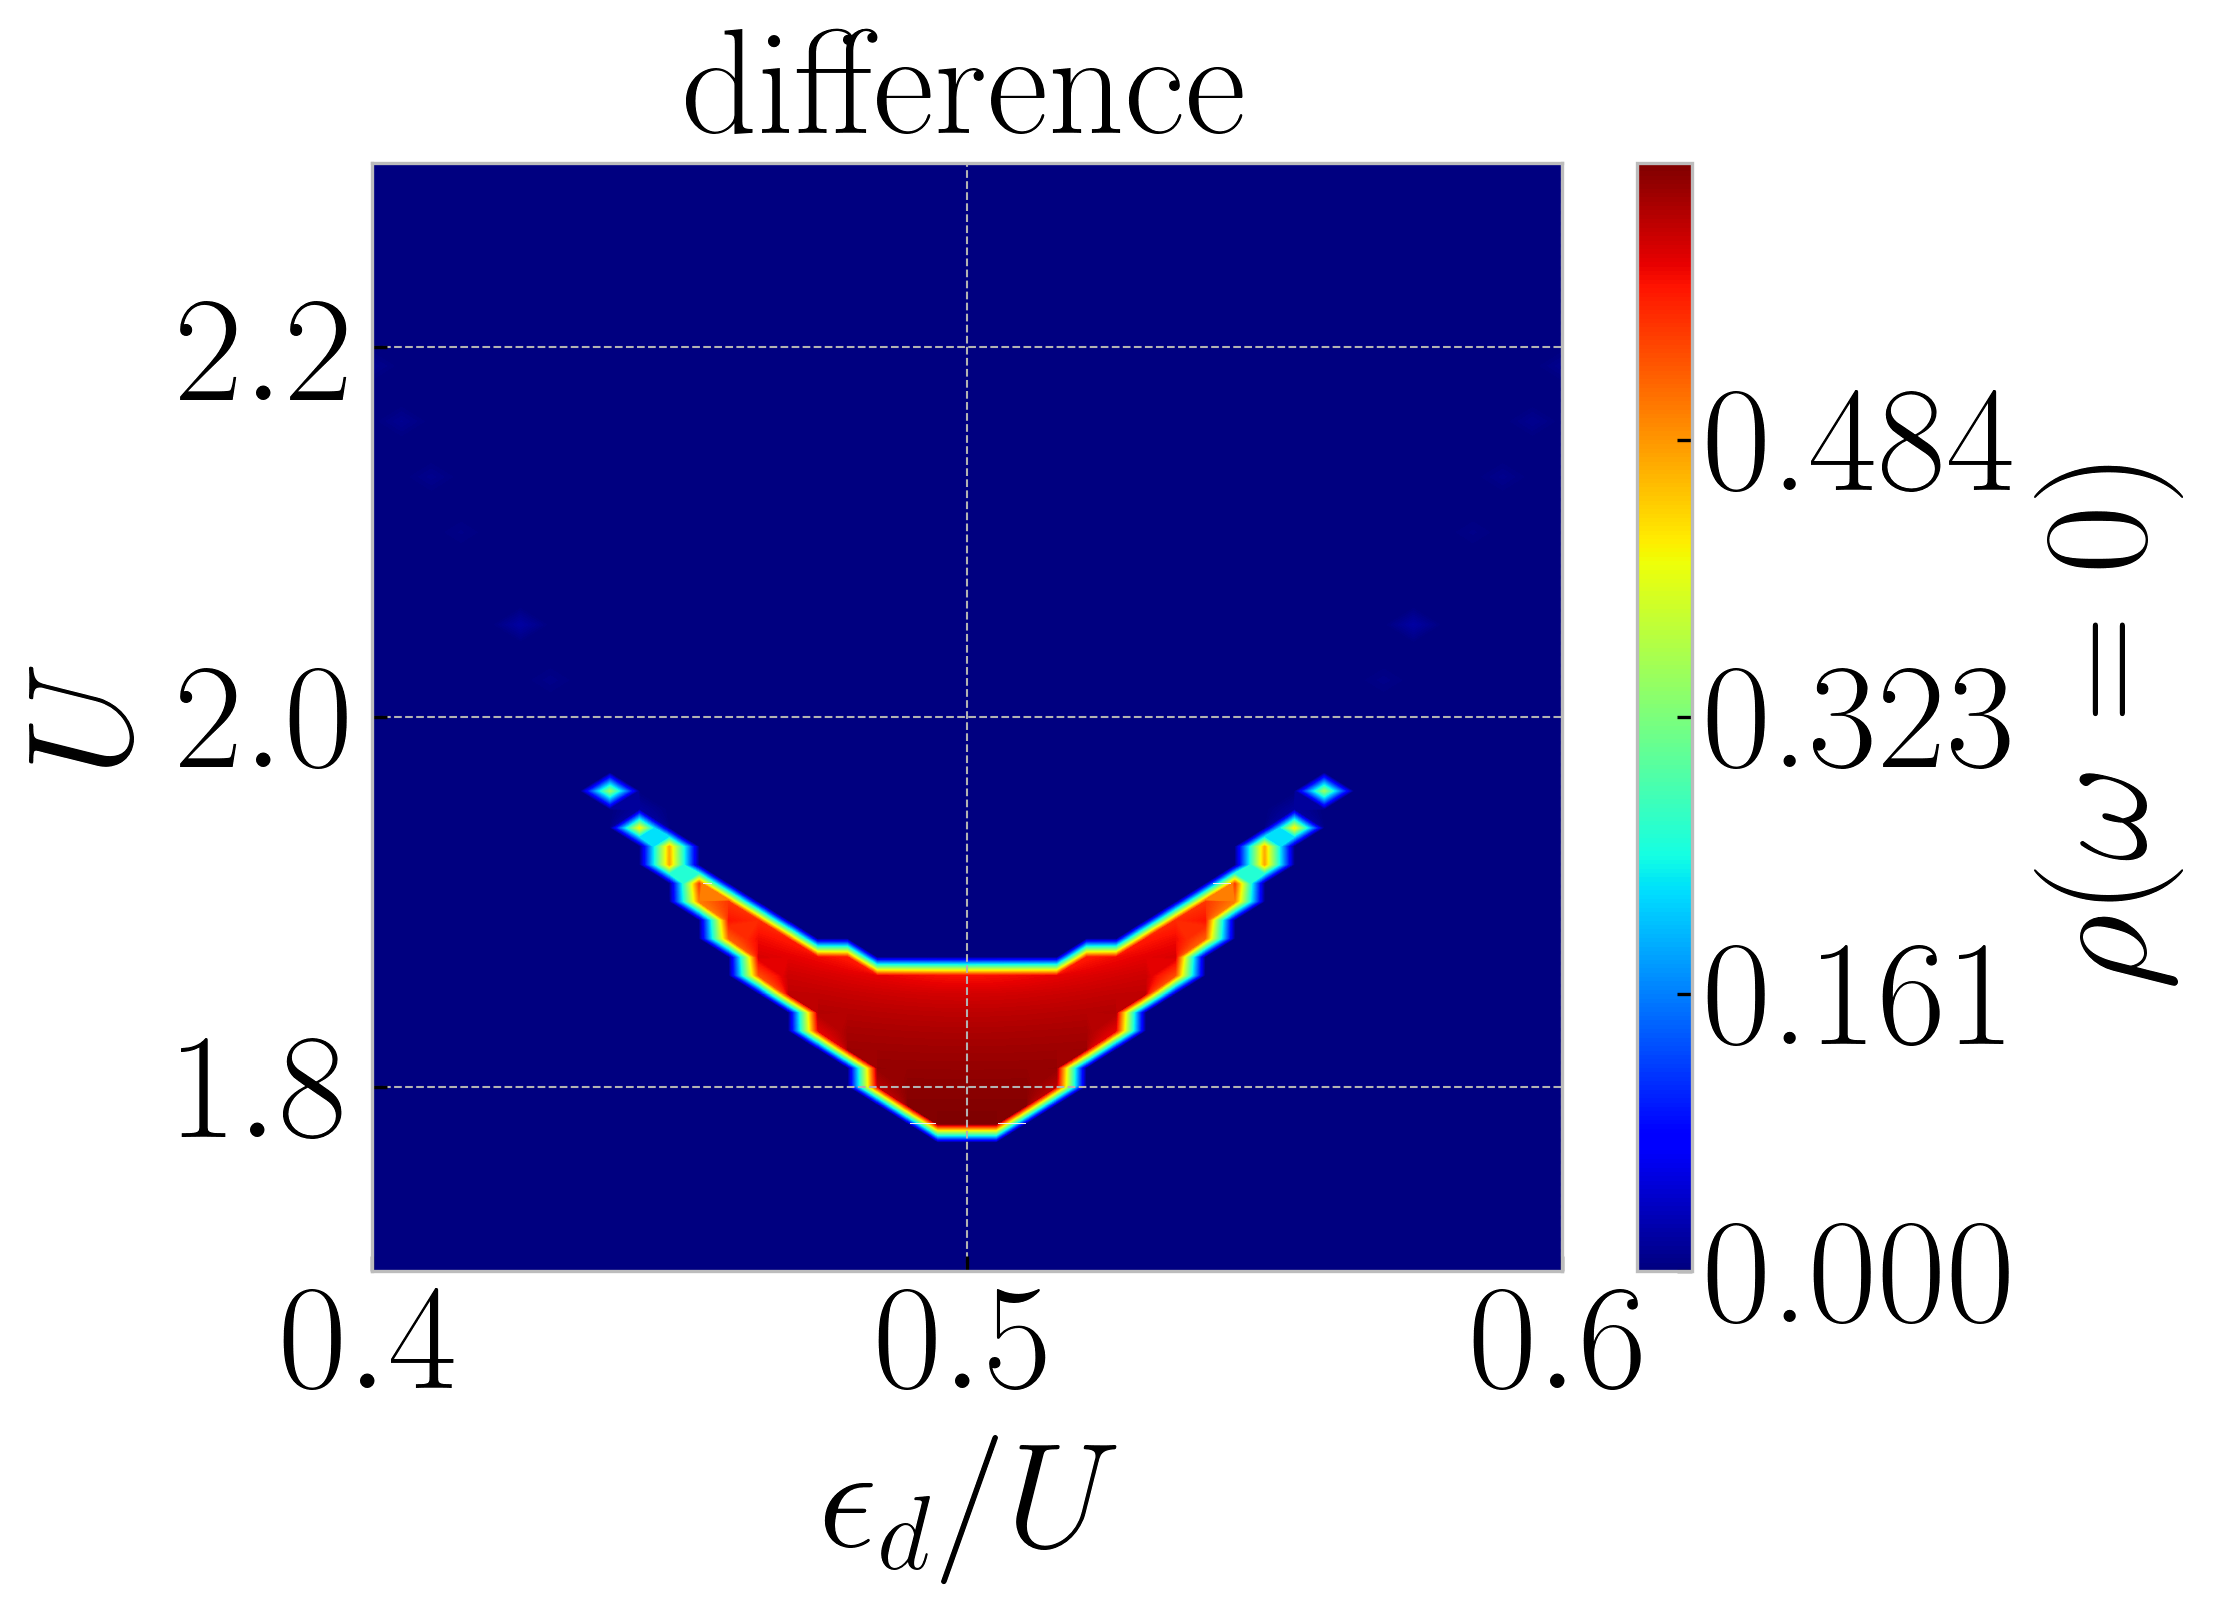
\includegraphics[width=0.42\textwidth]{fig/dmft/fig_diffe-w0-T0002.png}
\hfill
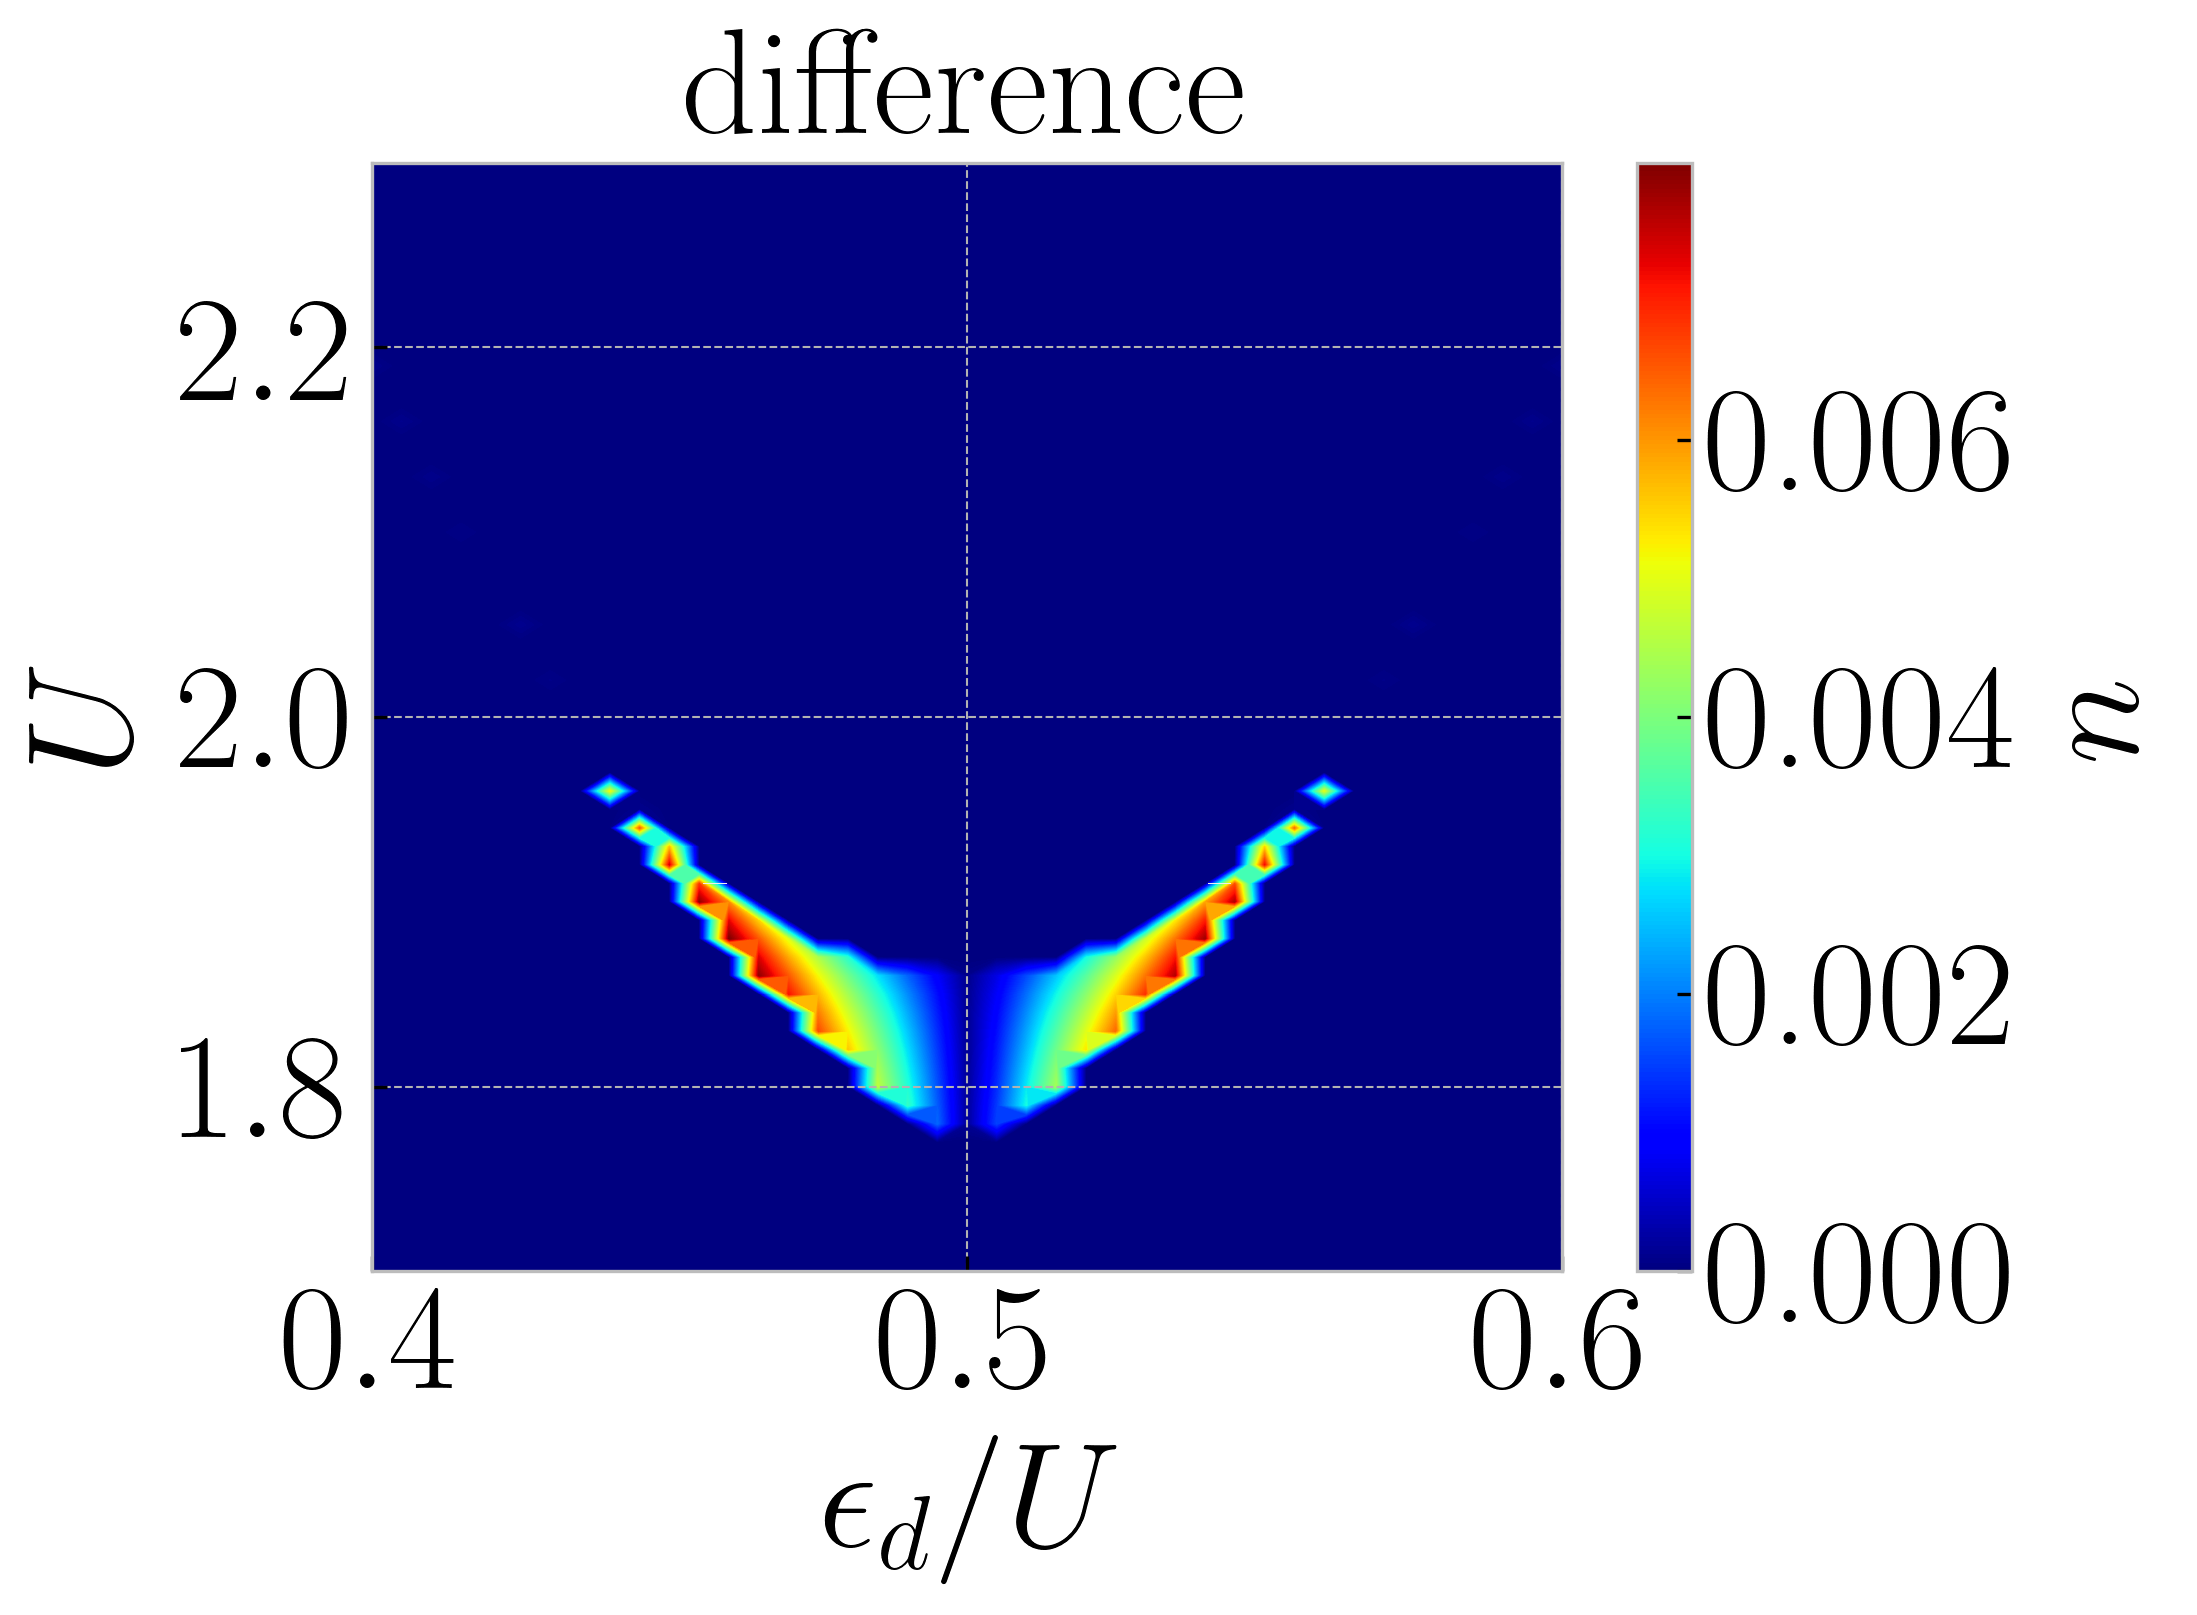
\includegraphics[width=0.42\textwidth]{fig/dmft/fig_diffe-nn-T0002.png}
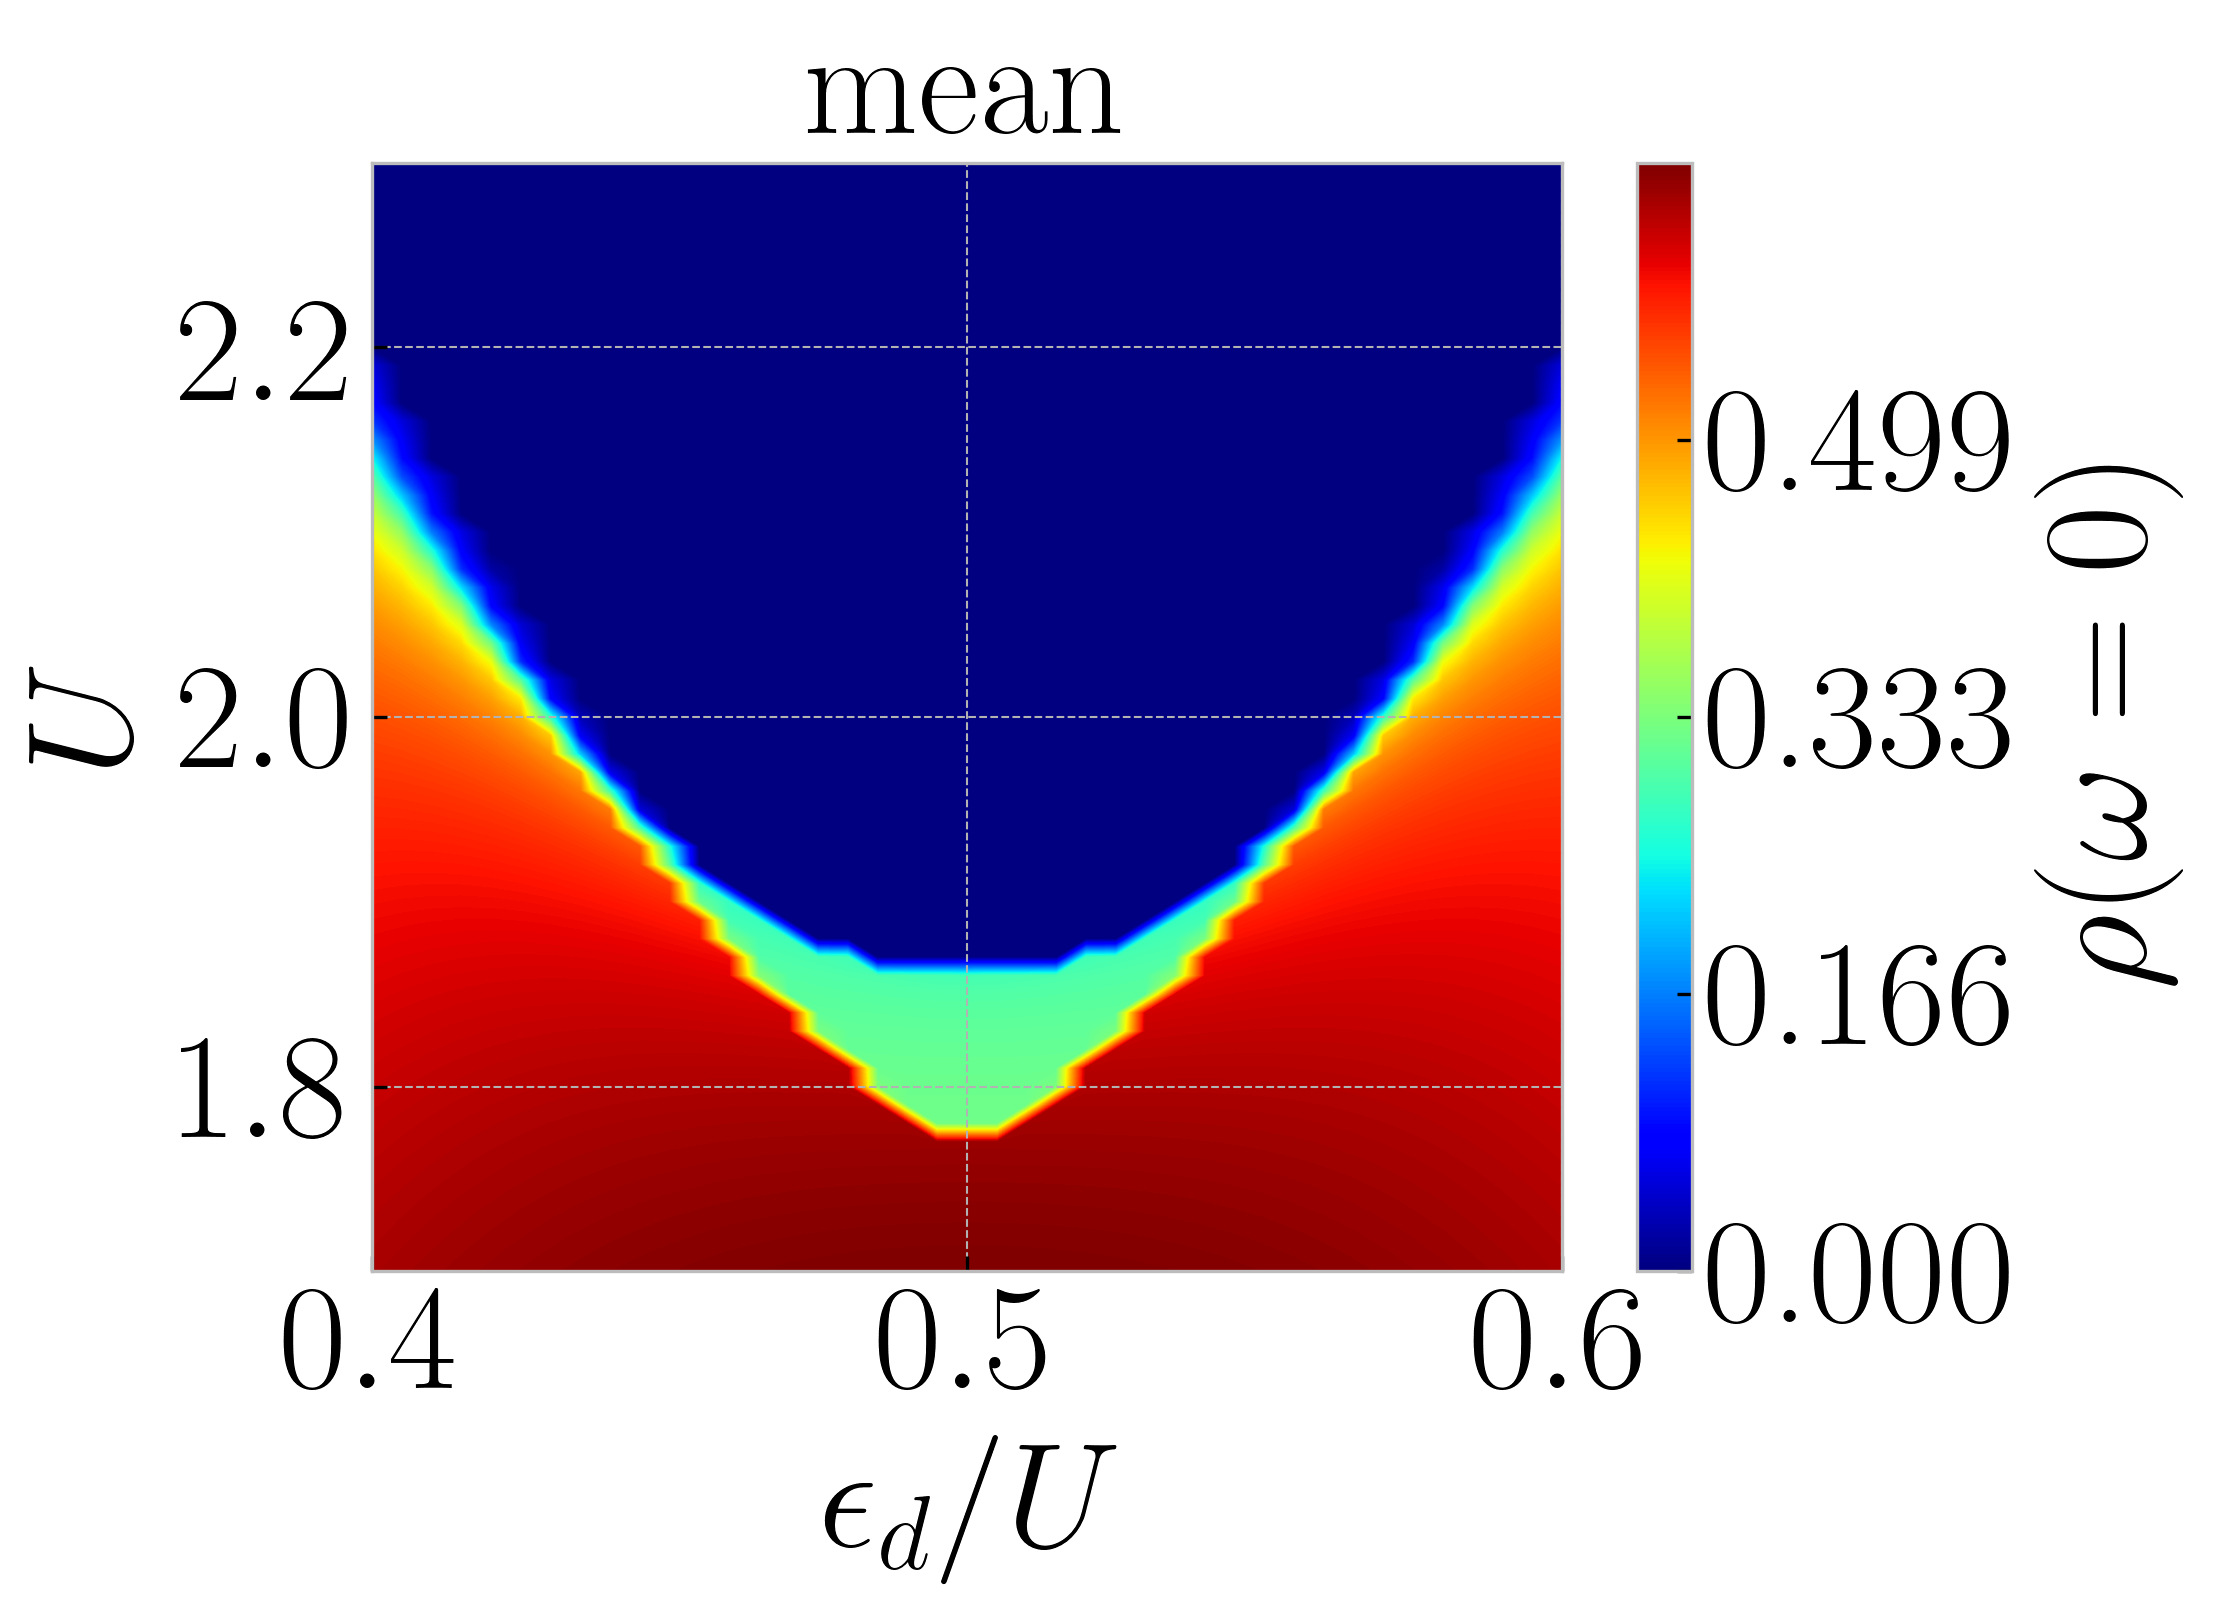
\includegraphics[width=0.42\textwidth]{fig/dmft/fig_mean2-w0-T0002.png}
\hfill
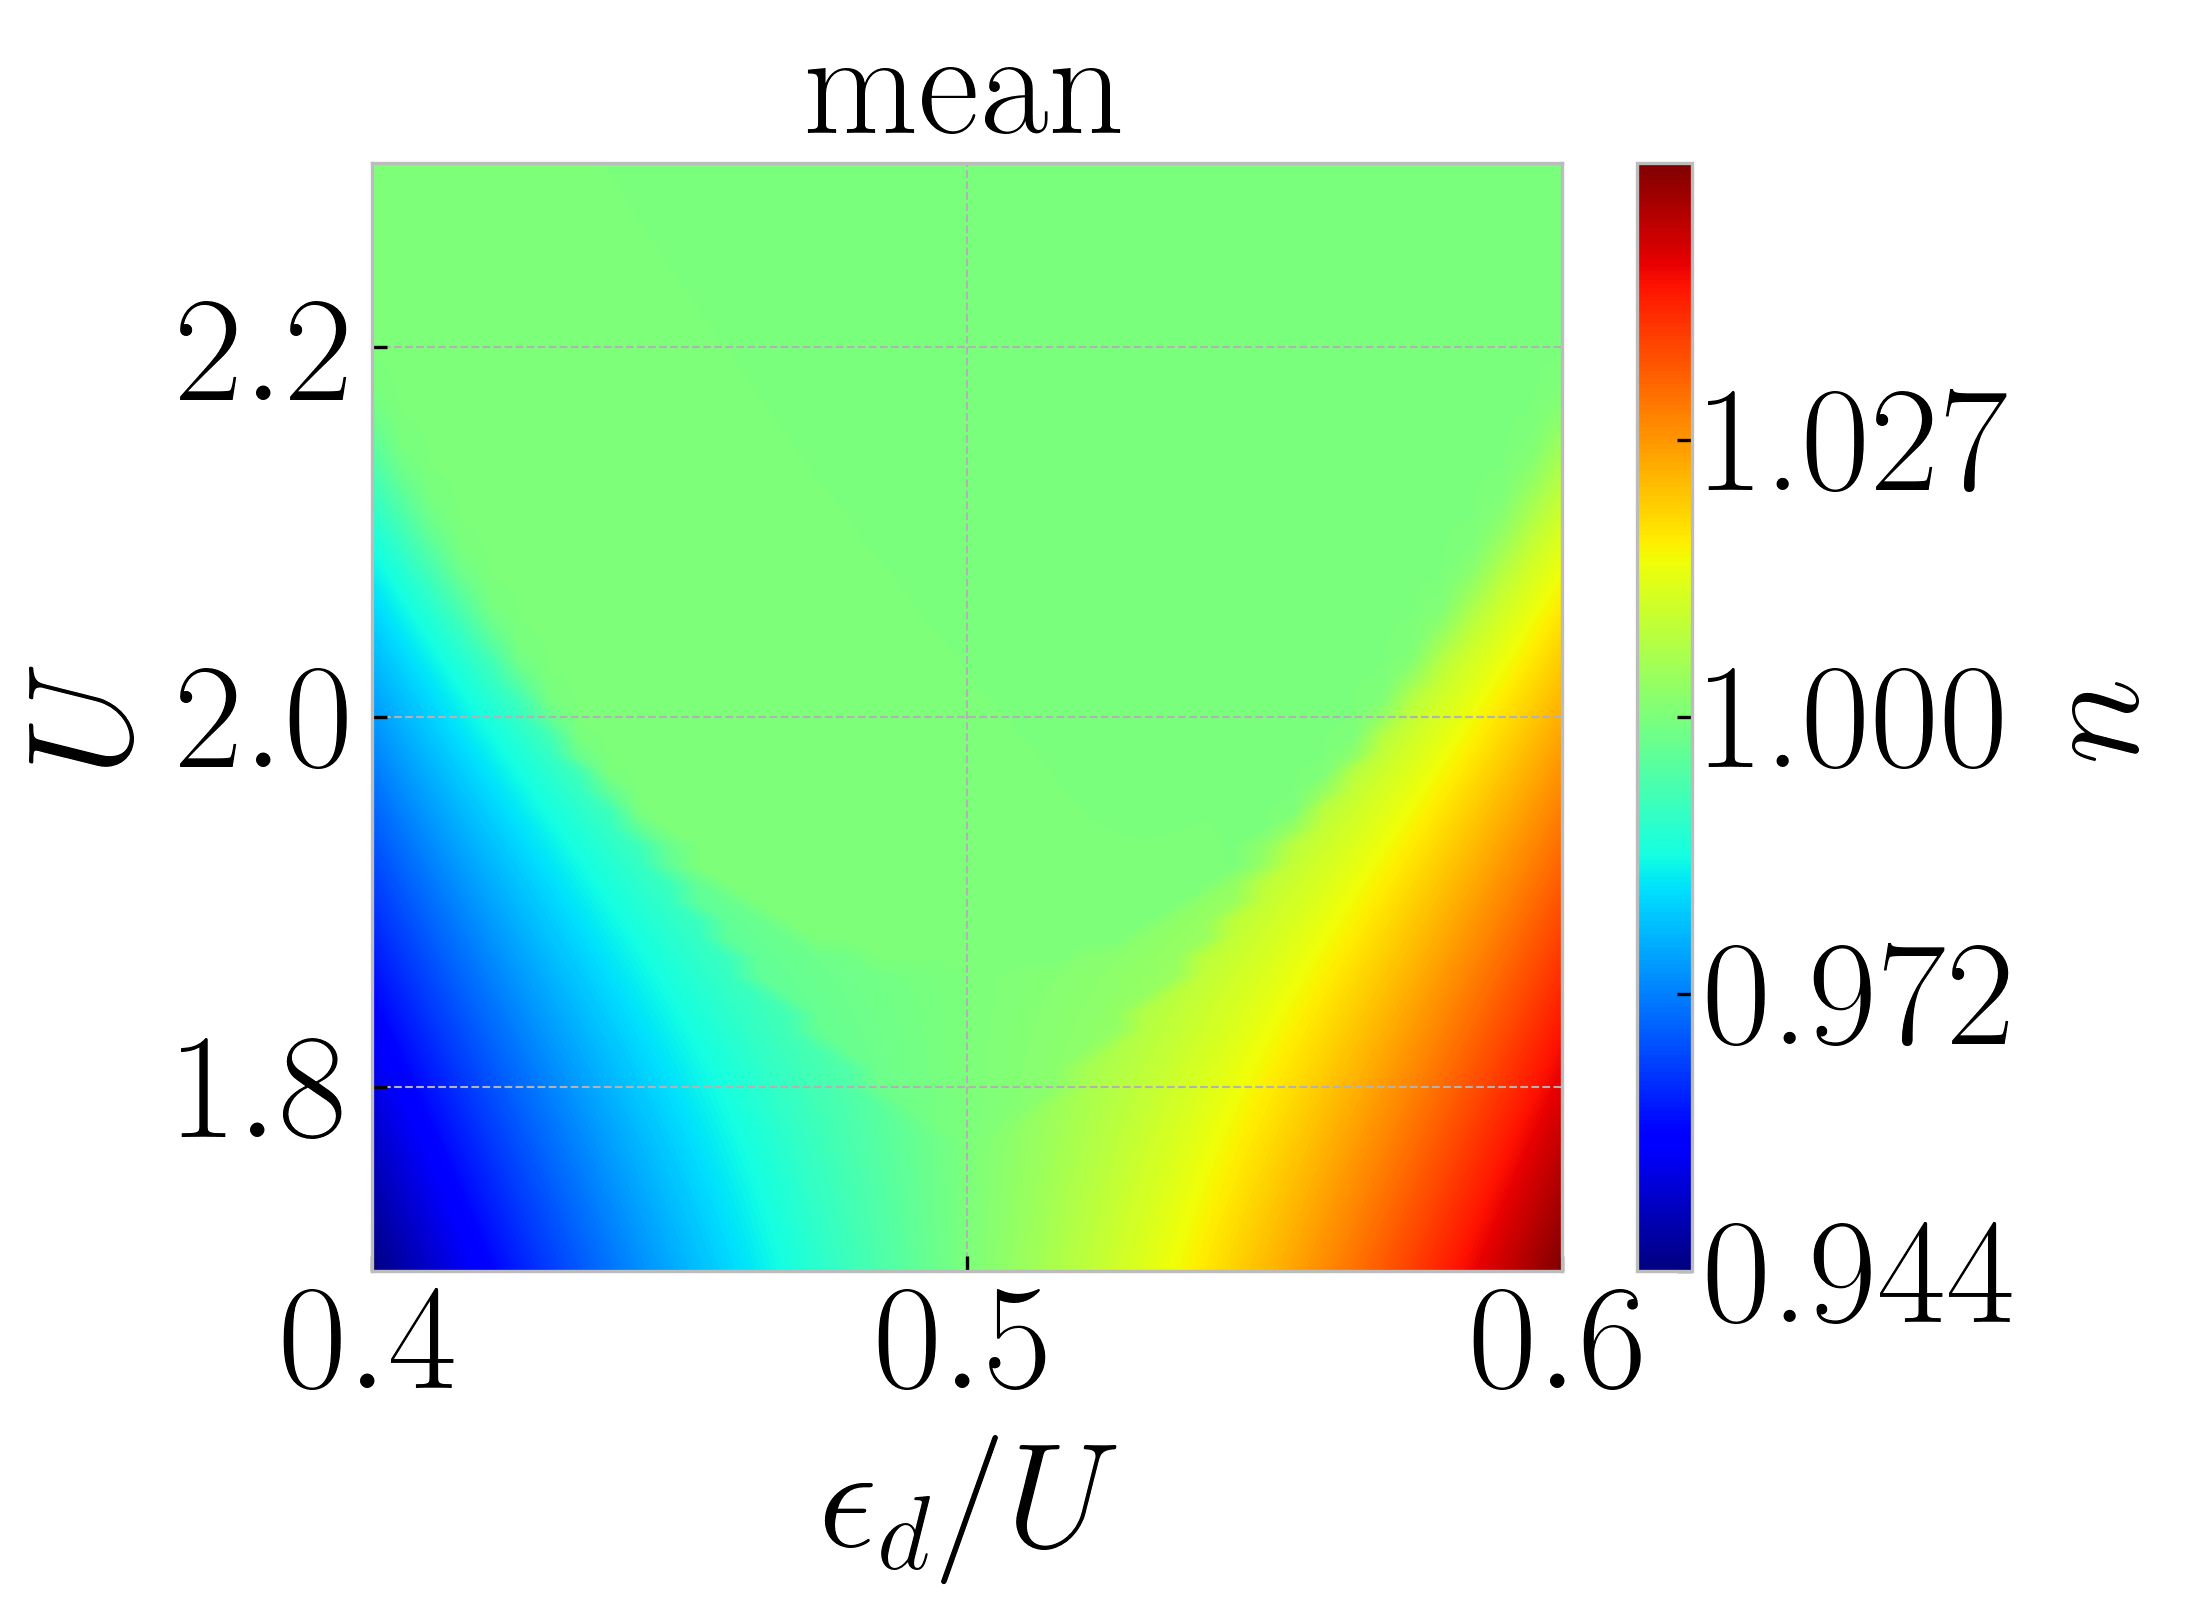
\includegraphics[width=0.42\textwidth]{fig/dmft/fig_mean2-nn-T0002.png}
\caption{Phase diagram  $U \times \epsilon_d$ for $T=0.002$. Panels labeled by ``difference'' (``mean'') show $\rho_{\text{diff}}$ ($\rho_{\text{mean}}$) and $n_{\text{diff}}$ ($n_{\text{mean}}$).}
\label{fig:Diagram_Drho_U_ed_T0002}
\end{figure}

Figure \ref{fig:Diagram_Drho_U_ed_T0002} show the $U \times \eps_d$ phase diagrams for a fixed temperature ($T = 0.002$), where we additionaly plot $\rho_{\text{diff}} = (\rho_{\text{metal}}(0) - \rho_{\text{insul}}(0))/2$ and $n_{\text{diff}} = (n_{\text{metal}} - n_{\text{insul}})/2$ to better visualize the distinction between the metal and insulator phases. It is interesting to notice the ``smile'' pattern formed by $\rho_{\text{diff}}$ and $n_{\text{diff}}$. In particular, the $n_{\text{diff}}$ panel shows that the two phases exhibit a difference of charge if the on-site energy (chemical potential) is fixed.

\section{Bilayer graphene} \label{sec:tbg}

\subsection{Monolayer graphene} \label{sec:monolayer}

Graphene is an allotrope of graphite and consists of a honeycomb lattice of carbon atoms linked in a $sp^2$ hybridization with a average distance $a = 0.246 \unit{nm}$, where three valence electrons from each carbon atom form $\s$ bonds and the last valence electron is located on a $\pi$ orbital and is the one that predominantly matters for the electronic properties of the material.

Figure \ref{fig:graphene-lattice_vectors} represents the honeycomb lattice structure of monolayer graphene, which can be seen as two hexagonal lattices $A$ (blue) and $B$ (yellow).

\begin{figure}[H]
\centering
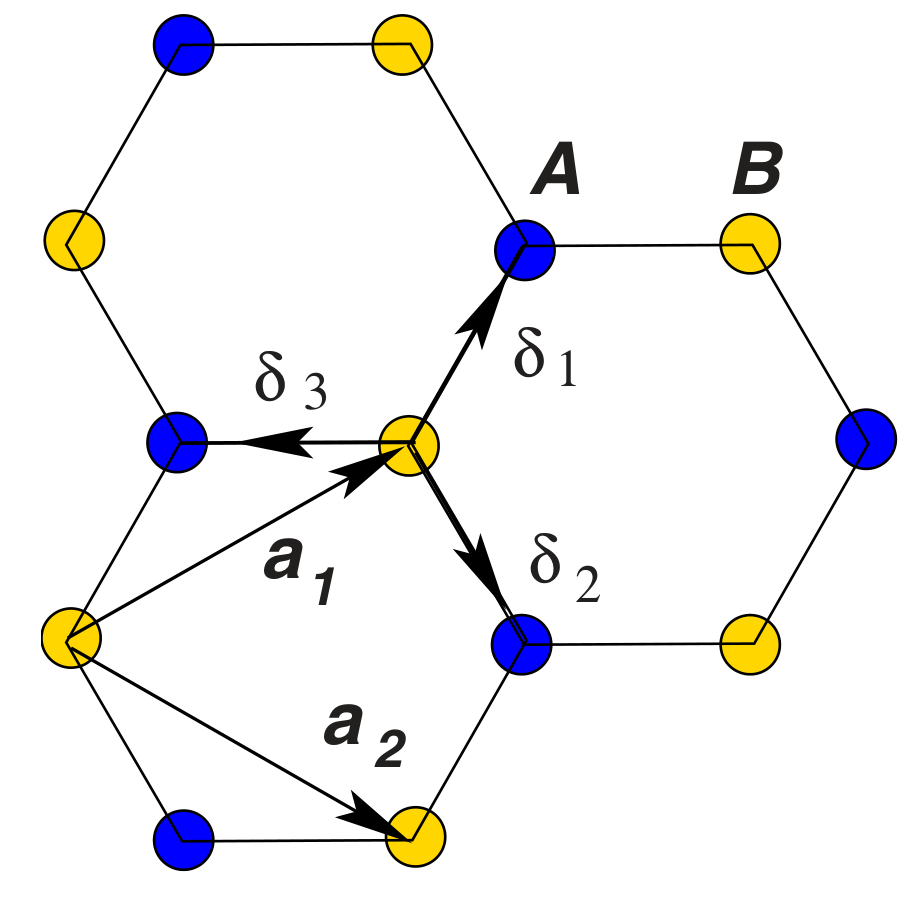
\includegraphics[width=0.4\linewidth]{fig/tbg/graphene-lattice_vectors.png}
\caption{Graphene's honeycomb lattice, its primitive vectors $\a_1$, $\a_2$ and nearest-neighbor vectors $\bm{\delta}_1$, $\bm{\delta}_2$ and $\bm{\delta}_3$. Figure taken from \cite{geim2009}.}
\label{fig:graphene-lattice_vectors}
\end{figure}

%The lattice vectors are $\vb{a}_1 = \frac{a}{2} (3, \sqrt{3})$, $\vb{a}_2 = \frac{a}{2} (3, -\sqrt{3})$ and the three nearest-neighbor vectors are $\bm{\delta}_1 = \frac{a}{2} (1, \sqrt{3})$, $\bm{\delta}_2 = \frac{a}{2} (1, -\sqrt{3})$, and $\bm{\delta}_3 = a (-1, 0)$.
%
%We write a tight-binding hamiltonian with only nearest-neighbor hopping
%$$
%H = -t \sum_{i,\nu} \qty(a^\d_{\r_i} b_{\r_i + \bm{\delta}_\nu} + h.c. ),
%$$
%where $\r_i$ runs through all sublattice $A$ sites, and $\nu = 1, 2, 3$. Applying the Fourier transforms
%$$
%a_{\r_i}^\d = \frac{1}{\sqrt{N}} \sum_{\k \in \text{BZ}} e^{-i \k \vdot \r_i} a_{\k}^\d,
%$$
%$$
%b_{\r_i} = \frac{1}{\sqrt{N}} \sum_{\k \in \text{BZ}} e^{i \k \vdot \r_i} b_{\k},
%$$
%we get
%$$
%H = \sum_{\k}
%\begin{pmatrix}
%a_{\k}^\d & b_{\k}^\d
%\end{pmatrix}
%\begin{pmatrix}
%0 & -t f(\k) \\
%-t f^*(\k) & 0
%\end{pmatrix}
%\begin{pmatrix}
%a_{\k} \\ b_{\k}
%\end{pmatrix},
%$$
%with
%$$
%f(\k) = \sum_{\nu} e^{i \k \vdot \bm{\delta}_\nu} =
%e^{-i k_x a} \qty[ 1 + 2 e^{-3ik_x a / 2} \cos(\sqrt{3} k_y a / 2) ].
%$$
%
%The eigenenergies of $h_{\k}$ (UNDEFINED yet) are $E_\pm(\k) = \pm t \abs{f(\k)}$.
%
%The roots of $f(\k)$ are given by solving $f(\k) = 0$, which gives us
%$$
%2 e^{-3ik_x a / 2} \cos(\sqrt{3} k_y a / 2) = -1 \implies
%\begin{cases}
%\; e^{-3i k_x a/2} = - 1, \\
%\; \cos(\sqrt{3} k_y a / 2) = \frac{1}{2}.
%\end{cases}
%\implies
%\begin{cases}
%\; k_x = \frac{2\pi}{3a}, \\
%\; k_y = \pm \frac{2\pi}{3 \sqrt{3} a},
%\end{cases}
%$$
%Therefore we define
%$$
%\K = \frac{2\pi}{3a} \qty(1, \frac{\sqrt{3}}{3}) \; \text{ and } \;
%\K' = \frac{2\pi}{3a} \qty(1, -\frac{\sqrt{3}}{3})
%$$
%which are the so-called Dirac points, around which the dispersion relation are approximately linear $E(\K + \q) = v_F \abs{\q} + O\qty[(\frac{q}{K})^2]$.



\subsection{Bernal (AB) stacking} \label{sec:ab-stacking}

The so-called Bernal or AB stacking of two layers of graphene is such that the atoms of sublattice $A$ from one layer are placed above the atoms of sublattice $B$ from the other layer.
To model the bilayer system in this configuration, we use the monolayer tight-binding hamiltonian (with only the first
nearest neighbors) as a basis and include an interlayer hopping \cite{handbook2019}. Indexing the layers with $\ell = 1, 2$, we write
\begin{equation} \label{eq:ab-hamil}
H = H_1 + H_2 + H_{\perp},
\end{equation}
\begin{equation} \label{eq:ab-slg-hamil}
\begin{split}
H_\ell &= -t \sum_{\R} c_{\ell,A}^\d(\R) [c_{\ell,B}(\R) + c_{\ell,B}(\R-\a_1) + c_{\ell,B}(\R-\a_2)] + \hc, \\
H_\perp &= t_{\perp} \sum_{\R} c_{1,A}^\d(\R) c_{2,B}(\R) + \hc,
\end{split}
%\begin{split}
%H_1 &= -t \sum_{\R} c_{1,A}^\d(\R) [c_{1,B}(\R) + c_{1,B}(\R-\a_1) + c_{1,B}(\R-\a_2)] + \hc, \\
%H_2 &= -t \sum_{\R} c_{2,A}^\d(\R) [c_{2,B}(\R) + c_{2,B}(\R-\a_1) + c_{2,B}(\R-\a_2)] + \hc,
%\end{split}
\end{equation}
where $t = 2.97 \unit{eV}$ is the monolayer graphene tight-binding's hopping, $t_\perp = 0.33 \unit{eV}$ is a homegeneous interlayer hopping \cite{handbook2019}, and $c_{\ell,\alpha}(\R)^\d$ is the creation operator for an electron in a state $\ket{\ell,\R,\alpha}$. Using the discrete Fourier Transform of the creation operators
\begin{equation} \label{eq:ft-creatio}
c_{\ell,\alpha}^\d(\R) = \frac{1}{\sqrt{N}} \sum_{\k\in\text{BZ}} e^{-i\k\vdot(\R+\bm{\tau}_{\ell,\alpha})} c_{\ell,\alpha}^\d(\k),
\end{equation}
we can rewrite $H = \sum_{\k} \Psi^\d(\k) H(\k) \Psi(\k)$, with $\Psi^\d(\k) = (c_{1,A}^\d(\k) \; c_{1,B}^\d(\k) \; c_{2,A}^\d(\k) \; c_{2,B}^\d(\k))$ and
\begin{equation} \label{eq:ab-momentum_space}
H(\k) =
\begin{pmatrix}
0 & -t f(\k) & 0 & t_\perp \\
-t f^*(\k) & 0 & 0 & 0 \\
0 & 0 & 0 & -t f(\k) \\
t_\perp & 0 & -t f^*(\k) & 0 \\
\end{pmatrix}.
\end{equation}

Diagonalizing $H(\k)$ we obtain the four bands for the AB-stacked bilayer graphene
\begin{equation} \label{eq:ab-four_bands}
E_{\pm,\pm}(\k) = \pm t
\sqrt{
\qty(\frac{t_\perp}{2t})^2 +
4 \cos(\frac{\sqrt{3}}{2} d \, k_x) \cos(\frac{3}{2} d \, k_y) + 2 \cos(\sqrt{3} d \, k_x) + 3
}
\; \pm \; \frac{t_\perp}{2}.
\end{equation}

Figure \ref{fig:ab-4bands} shows the plot of the dispersion relation in equation \ref{eq:ab-four_bands}.

\begin{figure}[H]
\centering
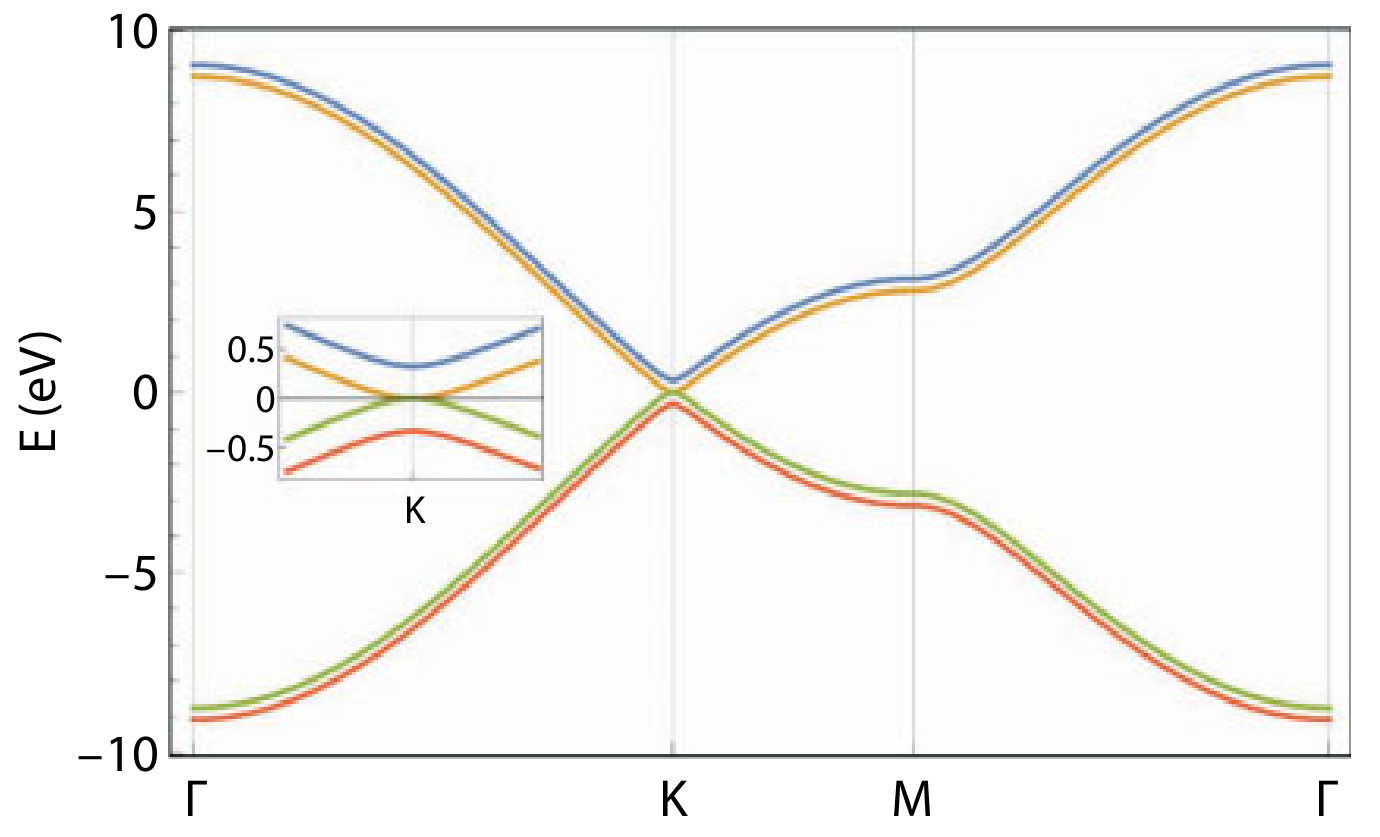
\includegraphics[width=0.6\linewidth]{fig/tbg/ab-4bands.png}
\caption{Four electronic bands for AB-stacked bilayer graphene obtained with tight-binding, along the $\k$-space trajectory $\Gamma \to K \to M \to \Gamma$. Figure taken from \cite{handbook2019}.}
\label{fig:ab-4bands}
\end{figure}

By implementing the BM model \cite{macdonald2011}, when we twist the two graphene layers (from the initial AB stacking) by a discrete set of very specific angles, with the first being $\theta \approx 1.05^\circ$, the bands in Figure \ref{fig:ab-4bands} should become very flat around the point $K$, which corresponds to the low-energy excitations of the system.


\subsection{TBG Geometry} \label{sec:tbg_geom}

The TBG system can be characterized by a rotation angle $\theta$ from the initial AB stacking stable setting. The two slightly misaligned layers then from an interference Moiré pattern, which can be commensurate (form a superlattice) or not. In the commensurate case, one can define primitive lattice vectors $\vb{L}_1$, $\vb{L}_2$ as the least common multiple of the unit vectors of two layers. Figure \ref{fig:latvec} shows an example of this.

\begin{figure}[H]
\centering
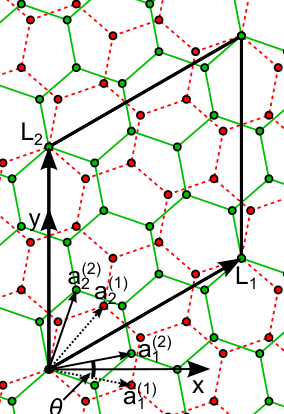
\includegraphics[width=0.4\textwidth]{fig/tbg/latvec.png}
\caption{Commensurate angle case and lattice vectors $\vb{L}_1$, $\vb{L}_2$. Figure taken from \cite{koshino2012}.}
\label{fig:latvec}
\end{figure}

As drawn in Figure \ref{fig:latvec}, we have
\begin{align}
\label{eq:scalarprods1}
\vb{a}_1^{(1)} \vdot \vb{a}_2^{(1)} &= a^2 \cos(60^\circ) = a^2/2; \\
\label{eq:scalarprods2}
\vb{a}_1^{(1)} \vdot \vb{a}_1^{(2)} &= a^2 \cos\theta; \\
\label{eq:scalarprods3}
\vb{a}_1^{(1)} \vdot \vb{a}_2^{(2)} &= a^2 \cos(60^\circ + \theta); \\
\label{eq:scalarprods4}
\vb{a}_1^{(2)} \vdot \vb{a}_2^{(1)} &= a^2 \cos(60^\circ - \theta).
\end{align}

The superlattice vectors $\vb{L}_1$, $\vb{L}_2$ are related by a $60^\circ$ rotation. In general, because $\vb{L}_1$ is a point that belongs to the lattices of both layers, it is written by integers $m,n,m',n'$ as
\begin{equation} \label{eq:L1}
\vb{L}_1 = m\vb{a}_1^{(1)} + n\vb{a}_2^{(1)} = m'\vb{a}_1^{(2)} + n'\vb{a}_2^{(2)}.
\end{equation}

Because there is an appropriate choice of lattice vectors $\vb{a}_1^{(1)}, \vb{a}_2^{(1)}, \vb{a}_1^{(2)}, \vb{a}_2^{(2)}$ (satisfying equations \ref{eq:scalarprods1} to \ref{eq:scalarprods4}) such that the indices $(m',n')$ can be made equal to $(n,m)$ \cite{koshino2012}, then by taking the scalar products of equation \ref{eq:L1} with $\vb{a}_1^{(1)}$ and $\vb{a}_1^{(2)}$, we get
\begin{equation} \label{eq:mn-system}
\begin{cases}
\; mn + n^2/2 = n^2 \cos\theta + mn \qty(\frac{\cos\theta}{2}
- \frac{\sqrt{3} \sin\theta}{2}); \\
\; m^2/2 + mn = m^2 \cos\theta + mn \qty(\frac{\cos\theta}{2}
+ \frac{\sqrt{3} \sin\theta}{2}).
\end{cases}
\end{equation}

Summing the two equations above gives us
\begin{equation} \label{eq:costheta}
\cos\theta = \frac{1}{2} \cdot \frac{m^2 + n^2 + 4mn}{m^2 + n^2 + mn}.
\end{equation}


By taking the norm of $\vb{L}_1$ from equation \ref{eq:L1} and using the angle relation in equation \ref{eq:costheta}, we find that the superlattice constant $L = \abs{\vb{L}_1} = \abs{\vb{L}_2}$ is given by
\begin{equation} \label{eq:}
L = a\sqrt{m^2 + n^2 + mn} = \frac{\abs{m-n}}{2 \sin(\theta/2)} \, a.
\end{equation}

The area of an unit cell of the superlattice is $A = \frac{\sqrt{3}}{2} L^2 = (m^2 + n^2 + mn) \, A_1$, where $A_1 = \frac{\sqrt{3}}{2} \, a^2$ is the area of unit cell of monolayer graphene. If we now consider the area of the Brillouin Zone (BZ), we get
\begin{equation} \label{eq:bz-volume}
\Omega = \frac{\Omega_1}{m^2 + n^2 + mn},
\end{equation}
where $\Omega_1 = (2\pi)^2/A$ is the BZ area of the monolayer and $\Omega$ is the area of the moiré mini BZ.

As an example, for $(m,n) = (1,2)$ we have $\theta = 21.8^\circ$ and $m^2 + n^2 + mn = 7$, therefore the monolayer BZ fits 7 mini BZ's in its area, as we see in Figure \ref{fig:bzminibz}.
\begin{figure}[H]
\centering
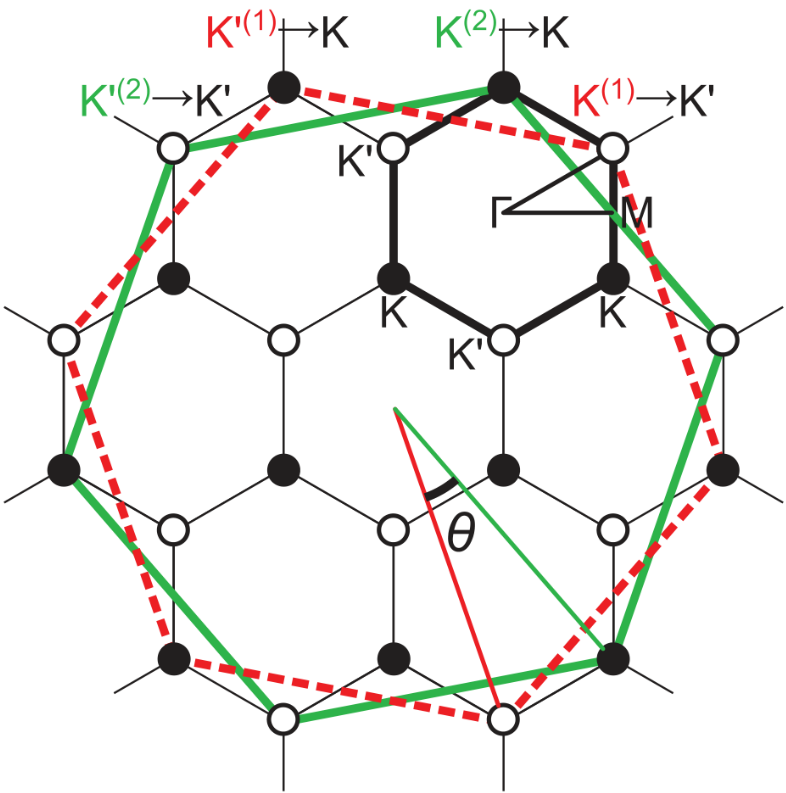
\includegraphics[width=0.5\linewidth]{fig/tbg/bzminibz.png}
\caption{Monolayers (red and green) and mini BZ's with $(m,n) = (1,2)$ and $\theta = 21.8^\circ$. Figure taken from \cite{koshino2012}.}
\label{fig:bzminibz}
\end{figure}

%%\pagebreak
%%\section{BM Model}
%%
%%Here we will review the Bistritzer-MacDonald (BM) model \cite{macdonald2011}. First of all, the moiré pattern can be interpreted by a beat effect. Define the functions $h_\ell(\r)$, for each layer $\ell = 1, 2$, that describe their periodicity
%%$$
%%h_\ell(\r) = \sum_{k=1}^{3} \cos(\vb{G}_{\ell,k} \vdot \r),
%%$$
%%where the wave vectors $\vb{G}_{\ell,1} = \vb{b}_{\ell,1}$, $\vb{G}_{\ell,2} = \vb{b}_{\ell,2}$ and $\vb{G}_{\ell,3} = \vb{b}_{\ell,1} - \vb{b}_{\ell,2}$ give the directions for nearest neightbor hoppings in the hexagonal lattice. The moiré pattern will then be an interference between $h_1(\r)$ and $h_2(\r)$,
%%$$
%%h_{\text{moiré}}(\r) = h_1(\r) + h_2(\r) =
%%\sum_{k=1}^{3}
%%\, 2 \cos(\frac{\vb{G}_{1,k}+\vb{G}_{2,k}}{2} \vdot \r) \cos(\frac{\vb{G}_{1,k}-\vb{G}_{2,k}}{2} \vdot \r).
%%$$
%%
%%The moiré pattern oscillates with $\vb{b}_k^{\text{moiré}} = \vb{G}_{1,k} - \vb{G}_{2,k}$, \cite{handbook2019}.
%%
%%Working on a coordinate system where the layer 2 is rotated by $\theta/2$ and layer 1 by $-\theta/2$, we have
%%$$
%%\vb{b}_1^{\text{moiré}} = \sqrt{3} \abs{\Delta K} \qty(\frac{1}{2}, -\frac{\sqrt{3}}{2}), \quad
%%\vb{b}_1^{\text{moiré}} = \sqrt{3} \abs{\Delta K} \qty(\frac{1}{2}, -\frac{\sqrt{3}}{2})
%%$$




\chapter{Evaluation of the Institutional Support received during the period} \label{chp:apoioInst}
%\chapter{Description and evaluation of the Institutional Support received during the period} \label{chp:apoioInst}

During the period covered by this report, the student used the Research Overhead to acquire the Acer Nitro 5 AN515-58-58W3 laptop, which was extensively used and very useful for the heavy DMFT calculations in Section \ref{sec:results}.



\chapter{Participation in scientific events} \label{chp:particEvento}

The student attended the following scientific events/courses as a listener:

\begin{itemize}
\item \href{https://www.ictp-saifr.org/qm2023/}{Workshop on Strong Electron Correlations in Quantum Materials: Inhomogeneities, Frustration, and Topology}.
\item \href{https://www.ictp-saifr.org/apsmarch23/}{APS/ICTP-SAIFR Satellite March Meeting}.
\item Journal Club of Luis Gregório G. V. Dias da Silva's research group.
\item \href{https://american-chemical-society.zoom.us/webinar/register/WN_FISEv0_ySkK2jPVB0nbsRw#/registration}{2023 ACS Communication and Scientific Writing Course}.
\item \href{https://uspdigital.usp.br/janus/componente/disciplinasOferecidasInicial.jsf?action=3&sgldis=PGF5891&idioma=en}{``Strong coupling theories for metal-insulator transitions: DMFT and beyond''} complementary course at USP.
\item Solid State I graduate course at USP.
\item Solid State II graduate course at USP.
\item Statistical Mechanics graduate course at USP.
\end{itemize}


\chapter{Conclusions and Future Activities} \label{chp:conclusions}

In Section \ref{sec:hubbard} we established a fully working DMFT algorithm and were able to explore the phase diagrams for the Metal-Insulator transition. In Figure \ref{fig:triangle-mu050} we could reproduce an already known result \cite{georges1996}, but we also investigated the asymmetric case, which is a little more obscure in the literature. In particular, in Figure \ref{fig:Diagram_Drho_U_T_coex} we were able to identify the growth of the coexistence region as $\eps_d$ approaches the symmetric case $U/2$ and the ``smile'' pattern in the $U \times \eps_d$ phase diagram in Figure \ref{fig:Diagram_Drho_U_ed_T0002}. With respect to our DMFT code, we expect to improve and extend the algorithm to multi-orbital systems in order to study the TBG.

In Section \ref{sec:tbg} we shared a little of what we studied about the TBG, but there is a lot more to understand. Firstly, we hope to fully understand the structure and implications of the BM model \cite{macdonald2011}. After that, we are going to focus on studying all the symmetries and topological issues in the topological heavy fermion model \cite{topoheavyfermion2022}. This will enable us to make progress on the practical DMFT implementation of TBG system.

%%-----
%% Referências bibliográficas
%%-----
\addcontentsline{toc}{chapter}{\bibname}
%\bibliographystyle{abntex2-num}
\bibliography{bibliografia}
\bibliographystyle{ieeetr}


%%-----
%% Fim do documento
%%-----

\end{document}
